\documentclass{pclass}
\usepackage [spanish] {babel} 
\usepackage[utf8]{inputenc}
\usepackage{eurosym}
\usepackage{graphicx}
\usepackage{float}
\usepackage{enumerate} 
\usepackage{url}
\begin{document}
\pagenumbering{arabic}
\tipo{Grado}   % Grado o M\'aster
\titulopro{Control de un coche mediante Raspberry Pi}
\tutor{Manuel Jesús Domínguez Morales}
\departamento{Arquitectura y Tecnología de Computadores}
%\autores{Nombre 1}{Nombre 2}  % Dos autores
\autores{Gonzalo Romero Castillo}{{\ }}   % Un autor
\dia{26 de Junio de 2017 (v.1.0)}
\titulacion{GITI}

\hacerportada

	\makeatletter
\renewcommand*\l@section{\@dottedtocline{1}{0em}{2.5em}}
\renewcommand*\l@subsection{\@dottedtocline{2}{1.5em}{3.2em}}
\renewcommand*\l@subsubsection{\@dottedtocline{3}{4.3em}{3.2em}}
\makeatother

\renewcommand{\frontmatter}{\pagenumbering{Roman}}
\frontmatter

\cdpchapter{Agradecimientos}

Mis más sinceros agradecimientos a:

\begin{itemize}
	\item Ángel Suárez Mora
	\item Francisco Javier Fernández Rodríguez
	\item Manuel Jesús Domínguez Morales
	\item Félix Romero Romero
	\item Petra Castillo Herrera
	\item Ángela Romero Castillo
	\item Juan Manuel Gutierrez Romero
	\item José Antonio (Villa)
	\item Antonio Cordero Sánchez
	
\end{itemize}
 
\cdpchapter{Resumen}

Este proyecto se enmarca en un entorno de hardware principalmente, en el que se pretende implementar el control total sobre un vehículo. En nuestro caso, se ha implementado el control manual de un vehículo prototipo, basado en un coche radio control ya que implementarlo en un coche real era costoso y peligroso. Este control se ha desarrollado en una aplicación para dispositivos basados en Android. Además, se quiso diseñar un sistema lo más modular posible y barato, con lo que desde un principio se adoptó la decisión de implementar el proyecto en torno al miniPC Raspberry Pi, en concreto la versión 3 modelo B. Después de varios fallos, se incluyó en el sistema un Arduino Nano para solucionar varios errores.

\medspace
\medspace
\medspace

Desde el primer momento se desarrolla el proyecto con la idea de automatizar el control del vehículo. Tras numerosos fallos y la falta de tiempo, se ha tenido que dejar la automatización completa en una pequeña parte de esta. Al principio se pensó en implementar el seguimiento de una línea mediante imágenes, pero al final se ha implementado una detección de personas que permiten la circulación o no del vehículo. En este caso, se ha desarrollado un script en PC el cual se encarga de la funcionalidad que acabamos de comentar.

\medspace
\medspace
\medspace

Con esto se pretendía desarrollar contenidos no vistos durante el Grado en Ingeniería Informática - Tecnologías Informáticas y además ahondar en el tema de control de automóviles. Además se pretendía aprender sobre el control de sistemas en tiempo real y obtener aptitudes que no se enmarcan en nuestros estudios en la universidad.



\cdpchapter{Resumen en inglés}

This project is framed in a hardware environment mainly, in which it is tried to implement the total control on a vehicle. In our case, we have implemented manual control of a prototype vehicle, based on a radio control car since implementing it in a real car was expensive and dangerous. This control has been developed in an application for devices based on Android. In addition, it was wanted to design a system as modular as possible and cheap, which from the beginning was adopted the decision to implement the project around the miniPC Raspberry Pi, specifically version 3 model B. After several failures, In the system an Arduino Nano to solve several errors.

\medspace
\medspace
\medspace

From the first moment the project is developed with the idea of automating the control of the vehicle. After numerous failures and lack of time, it has had to leave the complete automation in a small part of it. At first it was thought to implement the tracking of a line by means of images, but in the end it has been implemented a detection of people that allow the circulation or not of the vehicle. In this case, a script has been developed in PC which is in charge of the functionality that we just comment.

\medspace
\medspace
\medspace

This was intended to develop content not seen during the Grado en Ingeniería Informática - Tecnologías Informáticas and further delve into the subject of automobile control. In addition it was intended to learn about real-time systems control and to obtain skills that are not part of our university studies.
        
\tableofcontents


\listoffigures
\mainmatter  


\chapter{BLOQUE 1: DESCRIPCIÓN DEL PROYECTO}
\section{Introducción y motivación}

Como bien sabemos la automatización de los coches acarrea ventajas muy obvias en materia de seguridad, no nos referimos al coche autónomo sino a un programador de velocidad inteligente, un detector de fatiga, la alerta en el cambio involuntario de carril, etcétera. Este mercado será muy importante en los próximos años gracias al auge de coches más modernos y tecnológicos y en parte por el coche autónomo.

Hay informes que predicen que los sistemas de asistencia al conductor avanzados generarán un mercado de 102 mil millones de dólares para el año 2030, una cantidad muy alta cuyo objetivo es transmitir que será muy importante para los fabricantes. 

Un vehículo autónomo es un tipo de automóvil con los sensores, procesadores, software y actuadores necesarios para conducirse por sí mismo. De todos modos, que un coche u otro tipo de vehículo sea capaz de conducirse completamente solo, sin necesidad de un humano, no es tan fácil, ni barato, como puede parecer, así que los próximos años vamos a ver una llegada paulatina y progresiva de estos tipos de vehículos.

Esto significa que durante un tiempo veremos vehículos más o menos autónomos, dependiendo de cuánto sean capaces de hacer por sí solos, y de cuánto necesaria sea la intervención de un humano en la conducción. Es por eso que se habla de que hay varios niveles de conducción autónoma. Vamos a explicarlos mejor.

El primer organismo que realizó una clasificación de los distintos niveles de conducción autónoma fue la NHTSA en 2013. La NHTSA es la agencia federal que se encarga de velar por la seguridad de las carreteras y de los coches en EE.UU. Aproximadamente podríamos asociarla en España a la labor de la Dirección General de Tráfico, pero con un perfil más técnico.

La NHTSA creó una escala con cinco niveles de automatización, de 0 a 4, focalizándose principalmente en las capacidades del vehículo de conducirse por sí mismo. El carácter de esta escala de clasificación era el de servir de guía para que la Administración legislara la correspondiente normativa.

El nivel 0 se corresponde con ninguna automatización de la conducción (o sea, un coche convencional), y el nivel 4 se corresponde con una automatización completa de la conducción, sin responsabilidad alguna del conductor, y sin que sea necesario siquiera que haya un conductor en el vehículo.

También en 2013 se realizó una clasificación en Alemania, por parte del BASt, el Instituto Federal de Investigación de Carreteras. En esta también se recogían cinco niveles. Sin embargo no se emplean números para los diferentes niveles, como en la clasificación de la NHTSA o de la SAE (que explicaremos más adelante).

En la clasificación BASt los cinco niveles de conducción automatizada son: solo conductor, asistida, automatización parcial, automatización elevada y automatización completa.

En 2014 la SAE realizó su propia clasificación, diferente a la de la NHTSA, y también diferente a la de la BASt, realizadas ambas el año anterior. En este caso su escala tiene seis niveles de automatización, de 0 a 5, y se focaliza más en el nivel de atención e intervención del humano en la conducción.

La SAE es la sociedad de ingenieros automotrices. Nació en 1905 en EEUU con la intención de que los técnicos pudieran difundir ideas y conocer novedades, así como para promover estándares en la industria. Actualmente está presente en muchos otros países (aquí en España también).

El que durante unos años coexistieran varias escalas de clasificación de la conducción autónoma supuso más de una confusión acerca de qué nivel de conducción autónoma tenía tal o cual modelo de coche o prototipo.

Hoy en día se está extendiendo y aceptando cada vez más el estándar creado por la SAE, de hecho la NHTSA ha adoptado este sistema de clasificación en septiembre de 2016, abandonando el suyo propio. La OICA, Organización Internacional de Constructores de Automóviles, estaba empleando la clasificación de la BASt, pero ahora la ha adaptado introduciendo el nivel 3 de automatización condicionada, y pasando a considerar también 6 niveles de conducción autónoma, como la SAE.

Se podría decir que la OICA ha realizado una combinación y confluencia de ambas clasificaciones, pero alineándose un poco más con la clasificación de la SAE y aceptando múltiples conceptos que esta introduce.

Los niveles de conducción autónoma aparecen descritos, junto a otras consideraciones y definiciones, en el estándar SAE J3016, publicado por primera vez en enero de 2014, y cuya última revisión data del 30 de septiembre de 2016.

De acuerdo al estándar SAE J3016 de niveles de conducción autónoma, para clasificar cualquier tipo de vehículo hay cuatro aspectos fundamentales para determinar el nivel de automatización del mismo. Puede parecer un poco complejo y abstracto al principio, pero esto es así porque se ha intentado realizar una clasificación generalista y lo más universal posible, sin entrar en detalles específicos o nombres concretos.

\begin{itemize}
	\item Quién se encarga del movimiento del vehículo (el humano o la máquina). El movimiento se diferencia entre longitudinal (o sea, acelerar y frenar) y lateral (o sea, la dirección).
	
	\item Quién se encarga de la detección y respuesta ante objetos y eventualidades (OEDR, por sus siglas en inglés), mediante sistemas que monitoricen el entorno del vehículo durante la conducción (el humano o la máquina).
	
	\item Quién se encarga del respaldo de la conducción, es decir, quién actúa en caso de fallo de los sistemas automatizados, o ante la pérdida de las condiciones para su funcionamiento (de nuevo, el humano o la máquina).
	
	\item Condiciones específicas para el funcionamiento del sistema (horarias, climatológicas, geográficas, tipo de carretera, cantidad de tráfico, velocidad, etc). Es decir, ¿el sistema de conducción automatizada funciona en todo caso, o solo en ciertas condiciones que lo limitan? (por ejemplo, si las líneas de carril están parcialmente borradas o no se ven bien, ¿sigue funcionando?, si hay niebla espesa, ¿sigue funcionando?, si la región no cuenta con mapas GPS fiables y precisos, ¿sigue funcionando?...). 
	
\end{itemize}

Además de esos cuatro aspectos fundamentales a tener en cuenta, el estándar J3016 se fija especialmente en el usuario de ese vehículo. Como hemos comentado antes, esta clasificación no entra en detalles acerca de qué tareas concretas es capaz de realizar el vehículo por sí mismo (por ejemplo: si reconoce peatones o no, si reconoce semáforos o no, si reconoce las señales de velocidad o no...).

En lo que se fija es en cuánto necesario es el humano durante la conducción del vehículo: si es muy necesario el vehículo tendrá un nivel de conducción autónoma bajo, y si no lo es para nada, desapareciendo por tanto la figura del conductor, entonces el vehículo tendrá un nivel de conducción autónoma alto.

Así que esta clasificación diferencia entre varios posibles usuarios de un vehículo:
\begin{itemize}
	\item Conductor: es decir, el que realiza en tiempo real las tareas de la conducción dinámica totalmente o en parte, y/o el respaldo a la conducción. Puede ser a su vez: conductor (convencional), que acciona los mandos y controles del vehículo manualmente, o bien conductor remoto, cuando no está sentado en la posición del conductor, pero acciona los mandos y controles del vehículo a distancia, a través de algún dispositivo de control remoto (por ejemplo para aparcar el coche sin estar dentro del mismo, a través de la llave del vehículo o de un teléfono).

	\item Pasajero: el usuario sin ningún papel en la operación del vehículo.

	\item Usuario preparado para intervenir: es decir, suya es la tarea del respaldo durante la conducción, y debe estar preparado para actuar inmediatamente en caso de fallo del sistema de conducción automatizada, o ante la pérdida de las condiciones necesarias para el funcionamiento, pasando en ese momento a ser conductor.

	\item Gestor, preparador o "despachador" del vehículo: el usuario que solo verifica que el sistema de conducción automatizada del vehículo está disponible y en condiciones correctas para funcionar, enciende y apaga el sistema y como mucho programa una ruta en el sistema de navegación GPS del vehículo. Esta figura está pensada por ejemplo para los vehículos autónomos de tipo robotaxi, donde un empleado en el aparcamiento de la flota de taxis autónomos envía a un cliente el robotaxi solicitado (de ahí este concepto de "despachar el coche", como si fuera un envío).


\end{itemize}

El estándar SAE J 3016, de "términos relacionados con los sistemas de automatización de conducción para vehículos de motor en carretera" establece seis niveles de conducción autónoma o automatización: de 0 (ninguna automatización) a 5 (vehículo completamente autónomo). Para cada nivel se indica la capacidad mínima que debe tener el vehículo con respecto a la automatización de funciones.

\begin{itemize}
	
	\item Nivel 0: No hay automatización de la conducción.
	
	\begin{itemize}
		\item Las tareas de conducción dinámica son realizadas completamente por el conductor (o sea, por el humano, como siempre).
	\end{itemize}

	\item Nivel 1: Asistencia al conductor.
	\begin{itemize}
		\item El vehículo cuenta con algún sistema de automatización de la conducción, ya sea para el control del movimiento longitudinal, ya sea para el control del movimiento lateral, pero no ambas cosas a la vez.
		
		\item El conductor (humano) sigue realizando el resto de tareas de la conducción.
		
		\item El sistema no cuenta con detección y respuesta ante objetos y eventualidades de manera completa, y esta tarea recae en el conductor (por ejemplo puede reconocer vehículos, pero no un animal que cruza la carretera).
		
		\item El funcionamiento del sistema está limitado a ciertas condiciones.
		
		\item El conductor sigue siendo conductor y debe estar atento a todo lo que sucede.
	\end{itemize}
	
	\item Nivel 2: Automatización parcial de la conducción.
	
	\begin{itemize}
		\item El vehículo cuenta con sistemas de automatización de la conducción tanto para el control del movimiento longitudinal, como para el control del movimiento lateral, ambos a la vez.
		
		\item El conductor (humano) ya no tiene que realizar tareas relativas al movimiento.
		
		\item El sistema no cuenta con detección y respuesta ante objetos y eventualidades de manera completa, y de nuevo esta tarea recae en el conductor.
		
		\item El funcionamiento del sistema sigue limitado a ciertas condiciones.
		
		\item El conductor sigue siendo conductor y debe estar atento a todo lo que sucede.
	\end{itemize}

	\item Nivel 3: Automatización condicionada de la conducción.
	
	\begin{itemize}
		\item El vehículo cuenta con sistemas de automatización de la conducción tanto para el control del movimiento longitudinal, como para el control del movimiento lateral, ambos a la vez.
		
		\item El sistema cuenta con detección y respuesta ante objetos y eventualidades de manera completa.
		
		\item En este nivel se habla de usuario preparado para intervenir si el sistema lo solicita o se produce un fallo o pérdida de las condiciones de funcionamiento, pasando a ser en ese momento conductor.
		
		\item El funcionamiento del sistema sigue limitado a ciertas condiciones.
		
		\item El conductor a veces lo es y a veces no.
	\end{itemize}

Para un coche con sistema de conducción automatizada de nivel 3, el estándar SAE J3016 establece que si se produjese un fallo del sistema, este debe informar al usuario de respaldo con tiempo suficiente para que pueda reaccionar adecuadamente e intervenir, mediante un mensaje o alerta de petición de intervención en la conducción.

	\item Nivel 4: Automatización elevada de la conducción.
	
	\begin{itemize}
		\item El vehículo cuenta con sistemas de automatización de la conducción tanto para el control del movimiento longitudinal, como para el control del movimiento lateral, ambos a la vez.
		
		\item El sistema cuenta con detección y respuesta ante objetos y eventualidades de manera completa.
		
		\item Ya no es necesario un usuario preparado para intervenir si el sistema lo solicita o se produce un fallo. El propio sistema de automatización de la conducción cuenta con un sistema de respaldo para actuar en caso de fallo del sistema principal y poder conducir hasta una situación de riesgo mínimo.
		
		\item Sin embargo el funcionamiento del sistema sigue limitado a ciertas condiciones y por tanto el vehículo puede encontrarse en situaciones en las que no pueda seguir conduciendo.
		
		\item Desaparece la figura del conductor.
	\end{itemize}

	\item Nivel 5: Automatización completa de la conducción.
	
	\begin{itemize}
		\item El vehículo cuenta con sistemas de automatización de la conducción tanto para el control del movimiento longitudinal, como para el control del movimiento lateral, ambos a la vez.
		
		\item El sistema cuenta con detección y respuesta ante objetos y eventualidades de manera completa.
		
		\item Ya no es necesario un usuario preparado para intervenir si el sistema lo solicita o se produce un fallo. El propio sistema de automatización de la conducción cuenta con un sistema de respaldo para actuar en caso de fallo del sistema principal y poder conducir hasta una situación de riesgo mínimo.
		
		\item No hay condiciones específicas limitantes para el funcionamiento del sistema, y por tanto el vehículo podría seguir conduciendo en todo momento o circunstancia.
		
		\item No es necesario el conductor.
	\end{itemize}

Tanto para el nivel 4 como para el nivel 5, puesto que no es necesario que haya un conductor, ni siquiera tampoco un usuario de respaldo, se podría prescindir de los elementos de control y manejo del vehículo: es decir, tendríamos vehículos sin volante ni pedales.

Para todos los niveles de automatización, incluso en los más altos, el estándar SAE J3016 recoge la posibilidad de que siga habiendo un conductor humano, si así lo desea el fabricante, y que este pueda activar o desactivar el sistema de conducción automatizada a voluntad, aunque técnicamente no sea necesario en ningún momento. \cite{cochesAutonomos}
\end{itemize}

\section{Objetivos del proyecto}
\section{Estado del arte}
El radio control nace en 1894 de la mano de Guillermo Marconi, el cual, realizó un experimento en el cual se accionaba una campanilla sin necesidad de hacer uso de un cable de cobre como en el telégrafo, muy usado en esa época. Este experimento no hubiese sido posible sin que antes otros científicos como Maxwell, teoría de la existencia de las ondas electromagnéticas, Hertz, experimentos centrados en la emisión de descargas, y Rumkorff no hubiesen descubierto los fenómenos de radiación e inducción.

En 1940, en plena II Guerra Mundial, surge un primer proyecto en el cual se dotaba a un avión de un sistema de radio-control La idea de aviones radio-dirigidos surge para intentar ahorrar vidas, ya que el avión, una vez puesto en el aire, era controlado desde tierra. Con el paso de los años, la mejora en los circuitos integrados y la miniaturización de estos, se incluye el radio-control en el modelismo. Aquí es donde este trabajo puede ser clasificado, en el modelismo de radio-control, aunque con algunos matices.

En el mercado existen infinidad de coches de modelismo radio-control controlados por una emisora y un receptor de ondas de radio. En este caso, se trata de un sistema en el que se utiliza la conectividad wifi para controlar el modelo, lo cual nos hace que el control pueda ser un dispositivo variable. Existen en el mercado algunos productos similares a este, como son modelos controlados desde un móvil a través de la conexión Bluetooth. La idea de este sistema es dotar al sistema de un sistema no tan rígido como un sistema de tiempo real, si no de un computador capaz de ser programado incluso para automatizar el control del modelo. A continuación mostramos varios productos ya existentes:



\begin{itemize}
    \item Spy Tank


\begin{figure}[H]
  \centering
    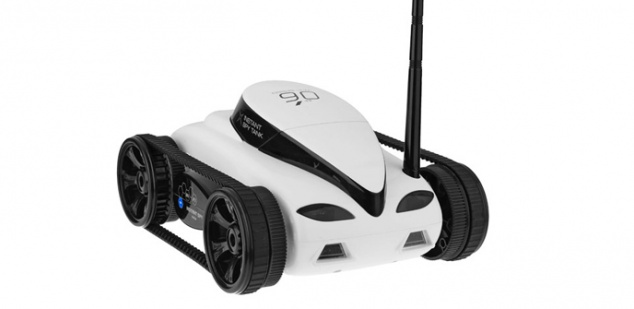
\includegraphics[width=1.1\textwidth]{img/producto1}
  \caption{Spy Tank}
  \label{fig:SpyTank}
\end{figure}



Este producto, el cual está diseñado para espiar, no para el disfrute del modelismo, tiene como puntos a favor que añade visión nocturna, cámara de visión con 360º, micrófono y altavoz. Tienen a su disposición sendas aplicaciones para Android e iOS, en las que con un uso sencillo de la interacción con la app es fácil controlar el coche, como por ejemplo con los acelerómetros Por contra, para el uso de este dispositivo necesitamos de una red wifi existente, ademas de su precio, unos 150 \euro más gastos de envío.



    \item BMW X6 Bluetooth
\end{itemize}

\begin{figure}[H]
  \centering
    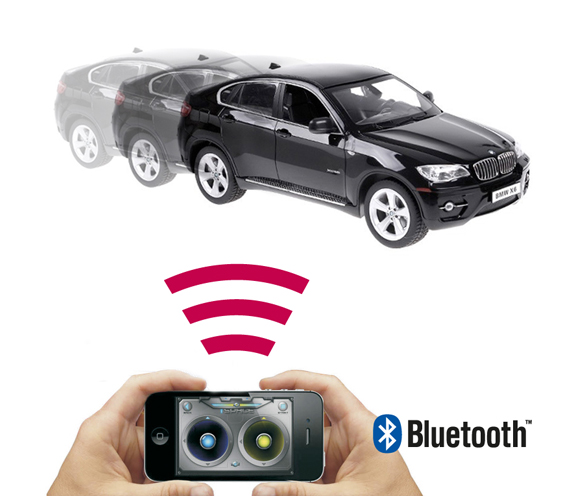
\includegraphics[width=1.1\textwidth]{img/producto2}
  \caption{BMW X6}
  \label{fig:BMWX6}
\end{figure}


Este producto se parece más a nuestro proyecto, podemos disfrutar del modelismo a un muy buen precio que ronda los 50 \euro. Simplemente nos encontramos con un coche que podemos controlar con sendas aplicaciones Android e iOS con la conexión Bluetooth. Por contra, no usa la red wifi, no tiene cámara de visión y además es tan simple que no podríamos implementar nada ya que no contiene ningún sistema programable con el que poder eliminar esa rigidez.



\section{Elicitación de requisitos y análisis de riesgos}


\chapter{BLOQUE 2: EJECUCIÓN DEL PROYECTO}
\section{Diseño del sistema}

La idea del proyecto es hacer un sistema barato y fácilmente adaptable a cambios en el vehiculo a controlar e incluso a cambios en el uso al que puede ser destinado. Además aprovecharemos la potencia que nos da el procesado de imágenes para tener control sobre el vehículo.

Para ello se va a usar un diseño modular, en el que cada parte se encarga de gestionar una pequeña parte de las funcionalidades que se ofrecen. En concreto Arduino se encarga de controlar dirección y acelerador/freno a través del variador y el servo. Raspberry por su lado, en comunicación con Arduino, se encarga de recibir comandos de un dispositivo externo y dar órdenes a Arduino para que este actúe. Además, emite en streaming las imágenes sacadas de la Webcam. 

Como aplicaciones que se han diseñado para controlar hay dos versiones, la versión sobre Android, que básicamente es una aplicación que recibe imágenes del Streaming y controla de forma manual el vehiculo y además, se ha diseñado un script para PC que procesa las imágenes del Streaming y decide si el vehículo puede continuar la marcha o no si detecta una persona en la imagen.

En la imágen que sigue se muestra a muy alto nivel los módulos de los que esta compuesto el proyecto.

	\begin{figure}[H]
		\centering
		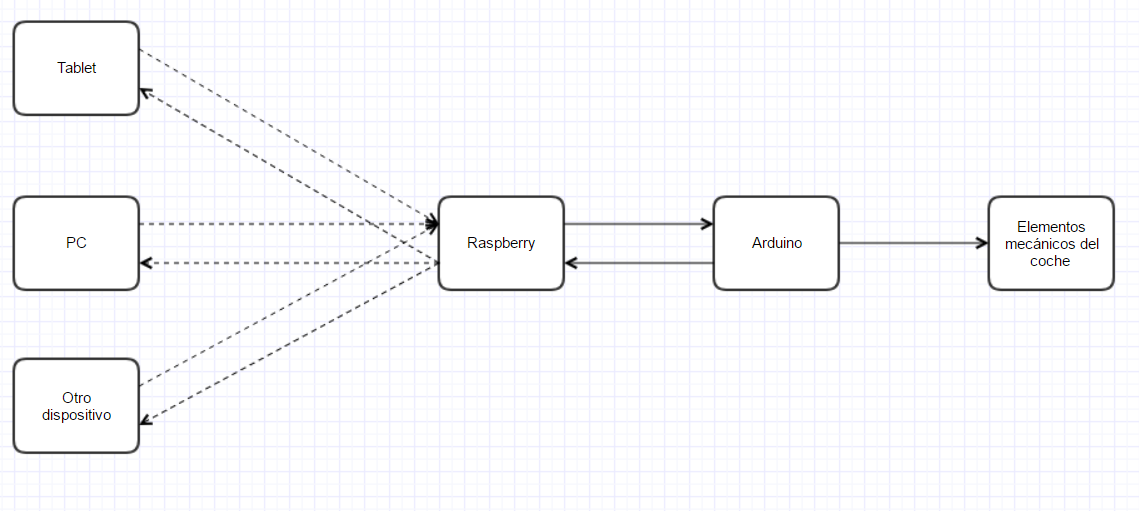
\includegraphics[width=0.90\textwidth]{img/diseno}
		\caption{Diagrama del diseño básico del proyecto}
		\label{fig:diseno}
	\end{figure}

En la imagen se aprecia que los dispositivos externos están unidos con líneas discontinuas, lo que indica es que la conexión a la Raspberry se hace mediante una red WiFi que emite la misma Raspberry. Esto se ha pensado para que el abanico de dispositivos externos no se vea limitado a una conexión física y además por la facilidad que da la comunicación mediante la red.

En los siguientes apartados se describirá más a fondo que hace cada parte y como se ha diseñado ya sea software o hardware.
 
\section{Implementación} 
\subsection{Tecnologías empleadas}

\begin{itemize}
	\item Hardware
		\begin{itemize}
			\item Raspberry Pi 3
			\item Arduino Nano
			\item Webcam
			\item Variador
			\item Servo
		\end{itemize}
	\item Software
	\begin{itemize}
		\item Mjpg Streamer
		
		MJPG-Streamer es un aplicación que se ejecuta por línea de comandos. A grandes rasgos, se encarga de obtener frames JPG (imágenes) capturadas desde una cámara compatible y transmitirlas como M-JPEG (secuencia de vídeo) mediante el protocolo HTTP para poder visualizarlo en navegadores, VLC y otras herramientas.
			\cite{mjpg}
		
		\item Hostapd y udhcpd
		
		Hostapd es un daemon para crear puntos de acceso y servidores de autentificación. Puede ser utilizado para crear puntos de acceso usando un ordenador con Linux. 
		
		Udhcpd es un pequeño servidor DHCP orientado a los sistemas embebidos.
		
			\cite{wireless}
		
		\item Raspbian	
		
		Raspbian es el sistema operativo oficial de la fundación Raspberry. Raspbian viene preinstalado con un montón de software para la educación, programación y uso general. Tiene Python, Scratch, Sonic Pi, Java, Mathematica y mucho más. En la versión lite no se usa interfaz gráfica.
		
			\cite{raspbian}
				
	\end{itemize}
	\item Lenguajes
		\begin{itemize}
			\item Python
			\item Arduino
		\end{itemize}
	\item Software de desarrollo
	\begin{itemize}
		\item Spyder
		\item Android Studio
		\item Arduino IDE
		\item Fritzing
		
		Fritzing es una iniciativa de hardware de código abierto que hace que la electrónica sea accesible como un material creativo para cualquiera. Ofrecemos una herramienta de software, un sitio web comunitario y servicios en el espíritu de Processing y Arduino, fomentando un ecosistema creativo que permite a los usuarios documentar sus prototipos, compartirlos con otros, enseñar electrónica en un aula y diseñar y fabricar PCB profesionales.
			\cite{fritzing}
		
		\item Tinkercad
		
		Tinkercad es una sencilla herramienta de diseño y modelado 3D basada en navegador que todos pueden usar. Tinkercad permite a los usuarios diseñar en cuestión de minutos todo lo que puedan imaginar.
			\cite{tinkercad}
			
		\item TeXstudio
		
		Texstudio es un entorno de escritura integrado para la creación de documentos LaTeX. Nuestro objetivo es hacer que la escritura del látex lo más fácil y cómoda posible. Por lo tanto texstudio tiene numerosas características como resaltado de sintaxis, visor integrado, verificación de referencias y varios asistentes.
			\cite{texstudio}
		\item Photoshop
		\item Gliffy
		
		Gliffy es una herramienta online que permite la creación de diferentes tipos de diagramas profesionales de forma sencilla.
			\cite{gliffy}
		
	\end{itemize}
\end{itemize}

 
\subsection{Desarrollo}

\begin{itemize}

\item Hardware y prototipo

En primer lugar, se llevó a cabo el desmontaje de las piezas innecesarias del prototipo, para sustituir las adecuadas para este sistema. En primer lugar se eliminó el antiguo receptor/variador para ser remplazado por un variador que controlase el motor sin ningún tipo de problemas. A esto se le sumó un problema, el servomotor que el prototipo traía era un motor eléctrico continuo, con lecturas de un potenciómetro, lo que después de muchas pruebas, tuvo que ser descartado dado que las lecturas del potenciómetro eran muy oscilantes e imposibilitaban el manejo correcto de la dirección. Siendo así, se sustituyo este servomotor, por un micro-servomotor normal, con el cual es mucho más fácil de trabajar.
A continuación se mostrará el coche sin ningún tipo de modificación:

\begin{figure}[H]
  \centering
    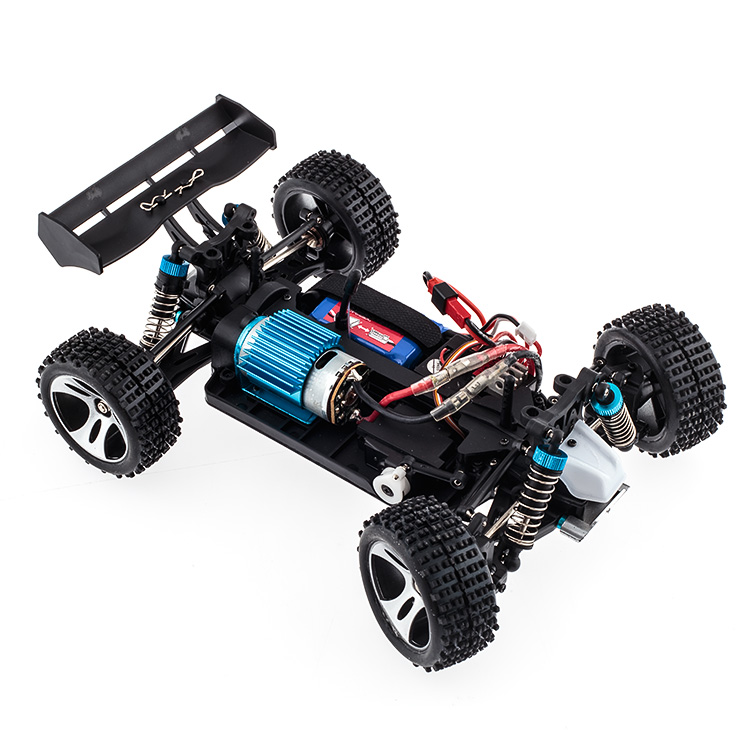
\includegraphics[width=0.7\textwidth]{img/A959}
  \caption{Coche sin desmontar}
  \label{fig:CocheSin}
\end{figure}

En la siguiente figura, se muestran las piezas eliminadas del prototipo:

\begin{figure}[H]
  \centering
    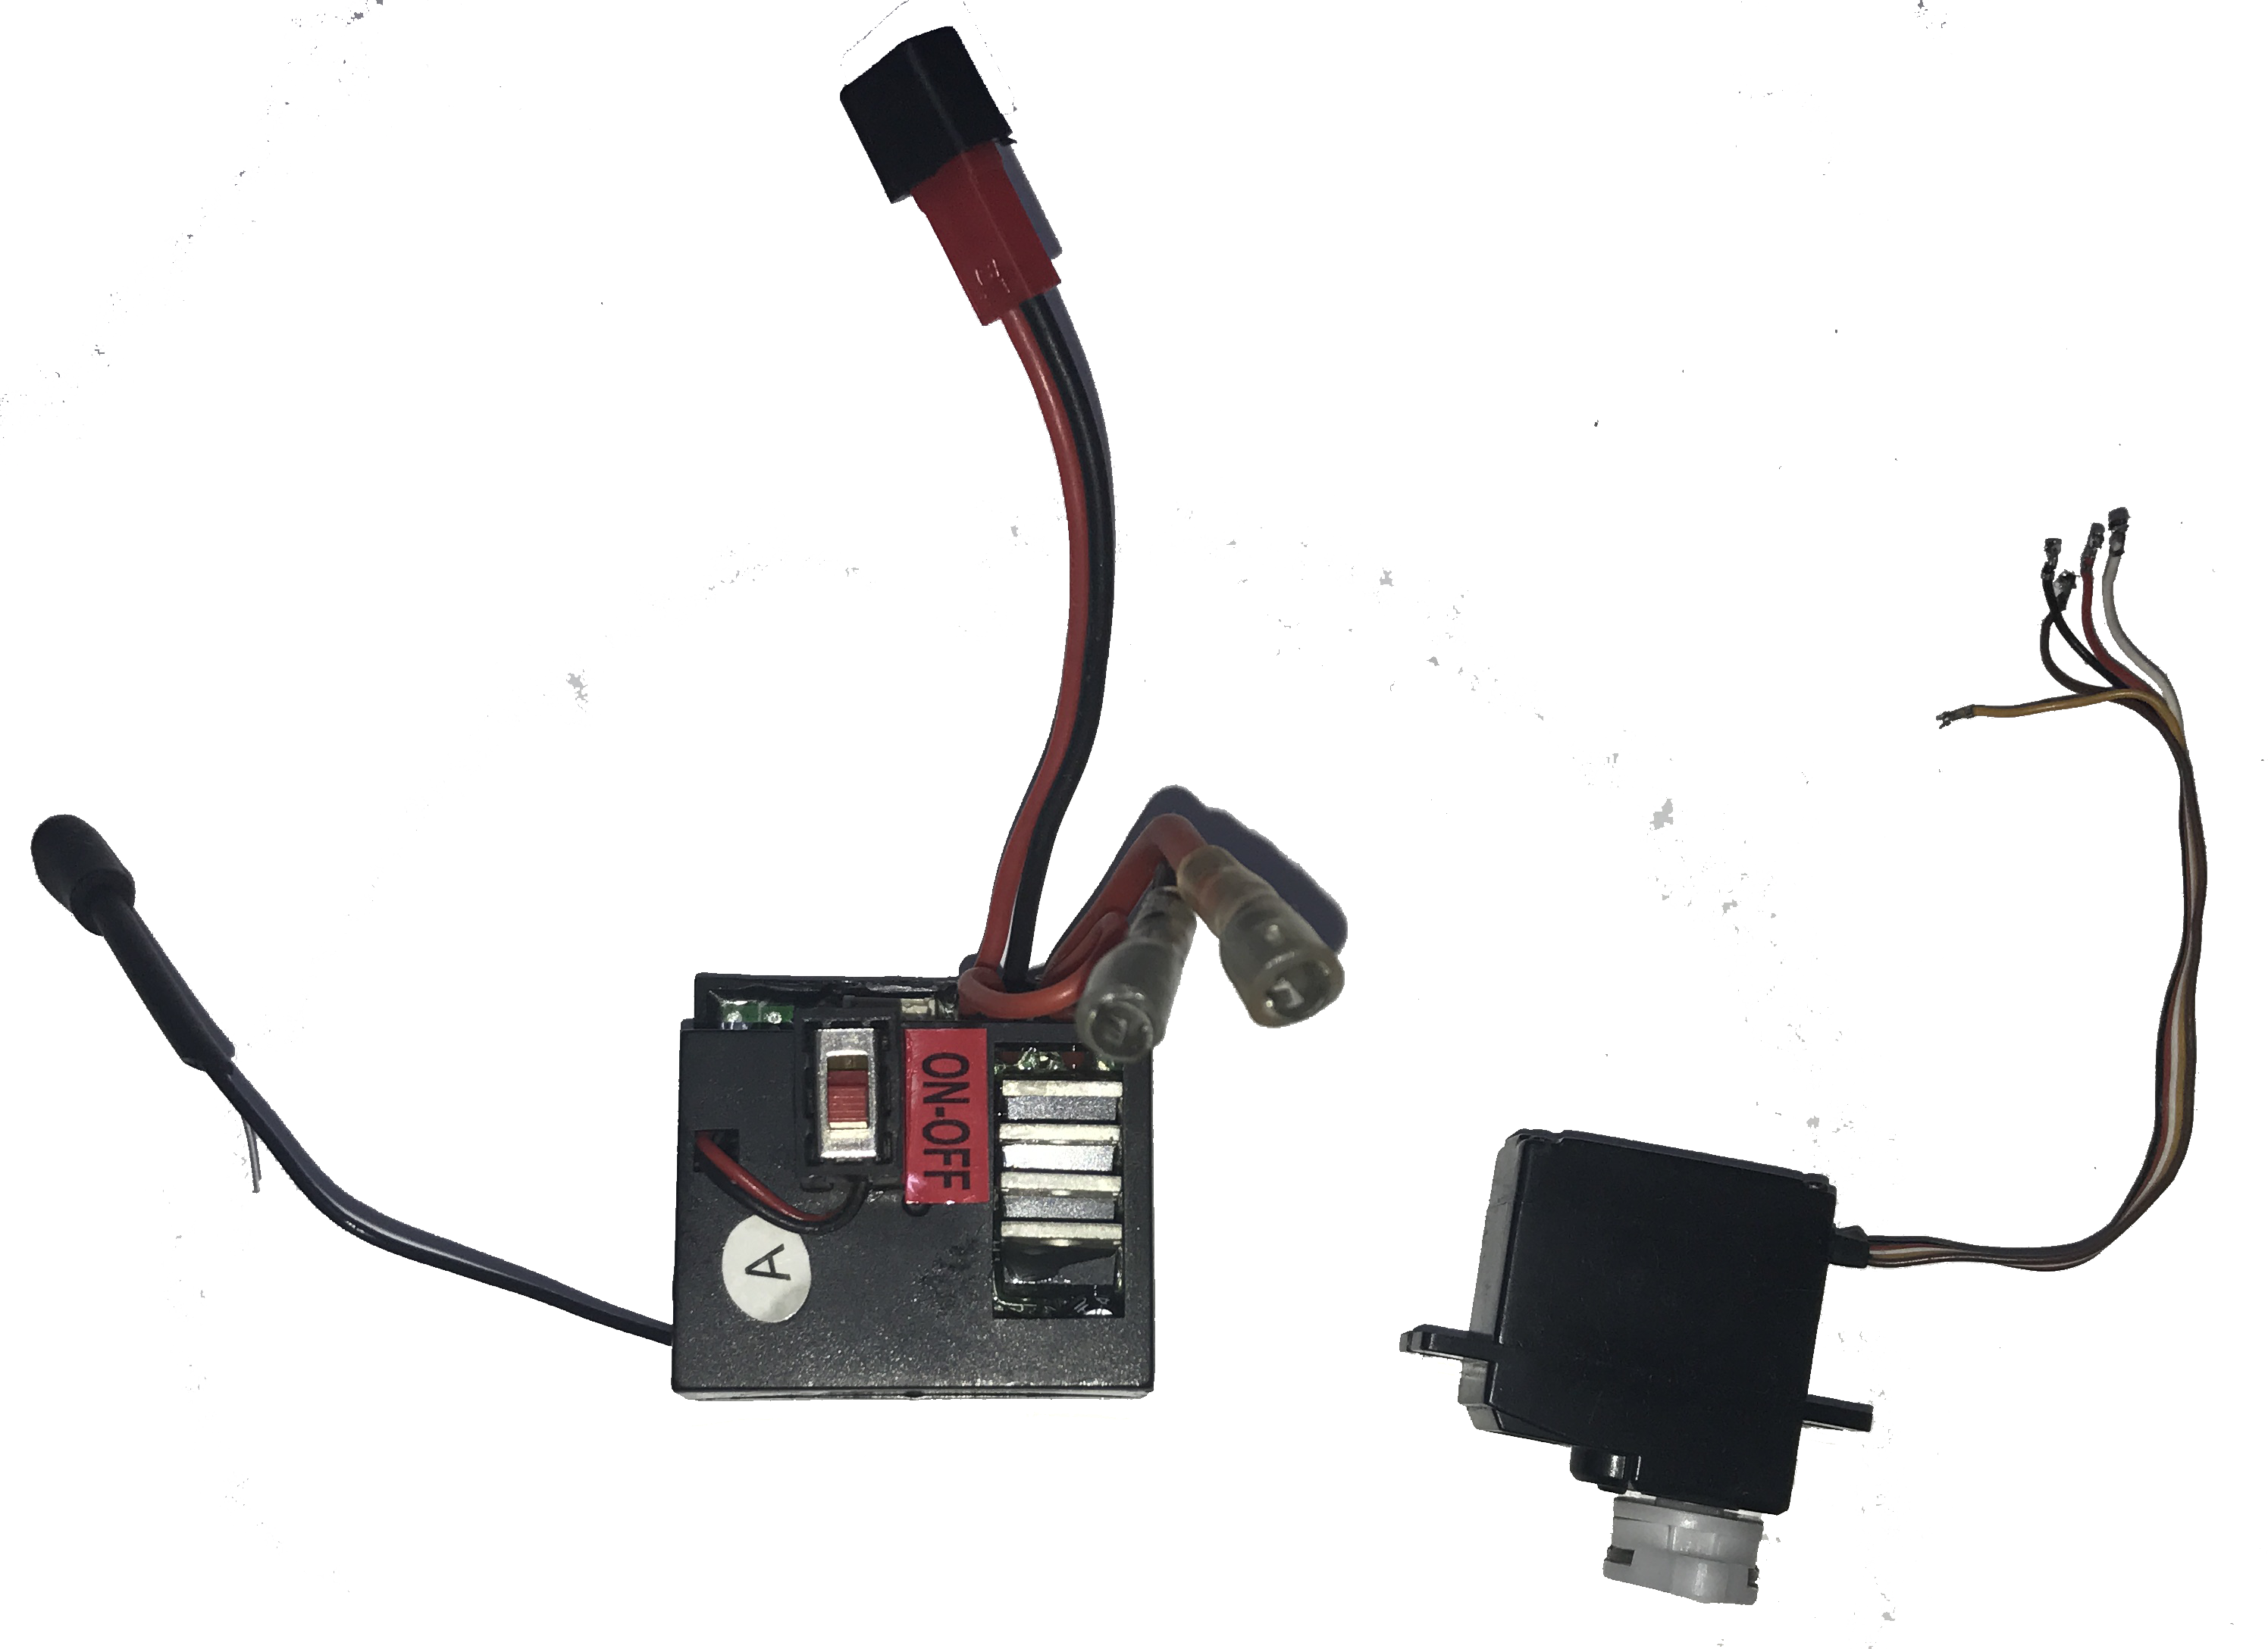
\includegraphics[width=0.7\textwidth]{img/piezasSustituidas}
  \caption{Piezas sustituidas}
  \label{fig:PiezasSusti}
\end{figure}

En la imagen que sigue, se muestra el prototipo con las nuevas piezas instaladas en su ubicación final. El variador lo encontramos en la parte frontal izquierda y el servomotor de la dirección en la parte frontal derecha, justo donde antes se ubicaban las piezas que eliminamos. El servomotor ha tenido que ser adaptado ya que las medidas del nuevo son más pequeñas. Además ha habido que adaptar el eje que transmite el movimiento a la dirección para que esta funcione correctamente.

\begin{figure}[H]
	\centering
	\includegraphics[width=0.7\textwidth]{img/piezasNuevas}
	\caption{Piezas nuevas en su ubicación}
	\label{fig:PiezasNuevas}
\end{figure}

En cuanto al hardware utilizado, inicialmente se planificó el uso de una Raspberry para todo el control del prototipo, pero después de varias pruebas con el sistema entrada/salida de la Raspberry y el motor y servo, se detectaron problemas con la generación de la señal PWM que controla estos, el cual no era estable y hacía que tanto el motor como el servo hicieran movimientos extraños. Esto suponemos que podría deberse a que la señal PWM pueda estar siendo generada por software. Como alternativa se ha optado por integrar un Arduino que se encargue de las funciones básicas de controlar tanto el servo como el motor. Para ello se ha conectado el Arduino a través de un cable USB a la Raspberry.

\begin{figure}[H]
	\centering
	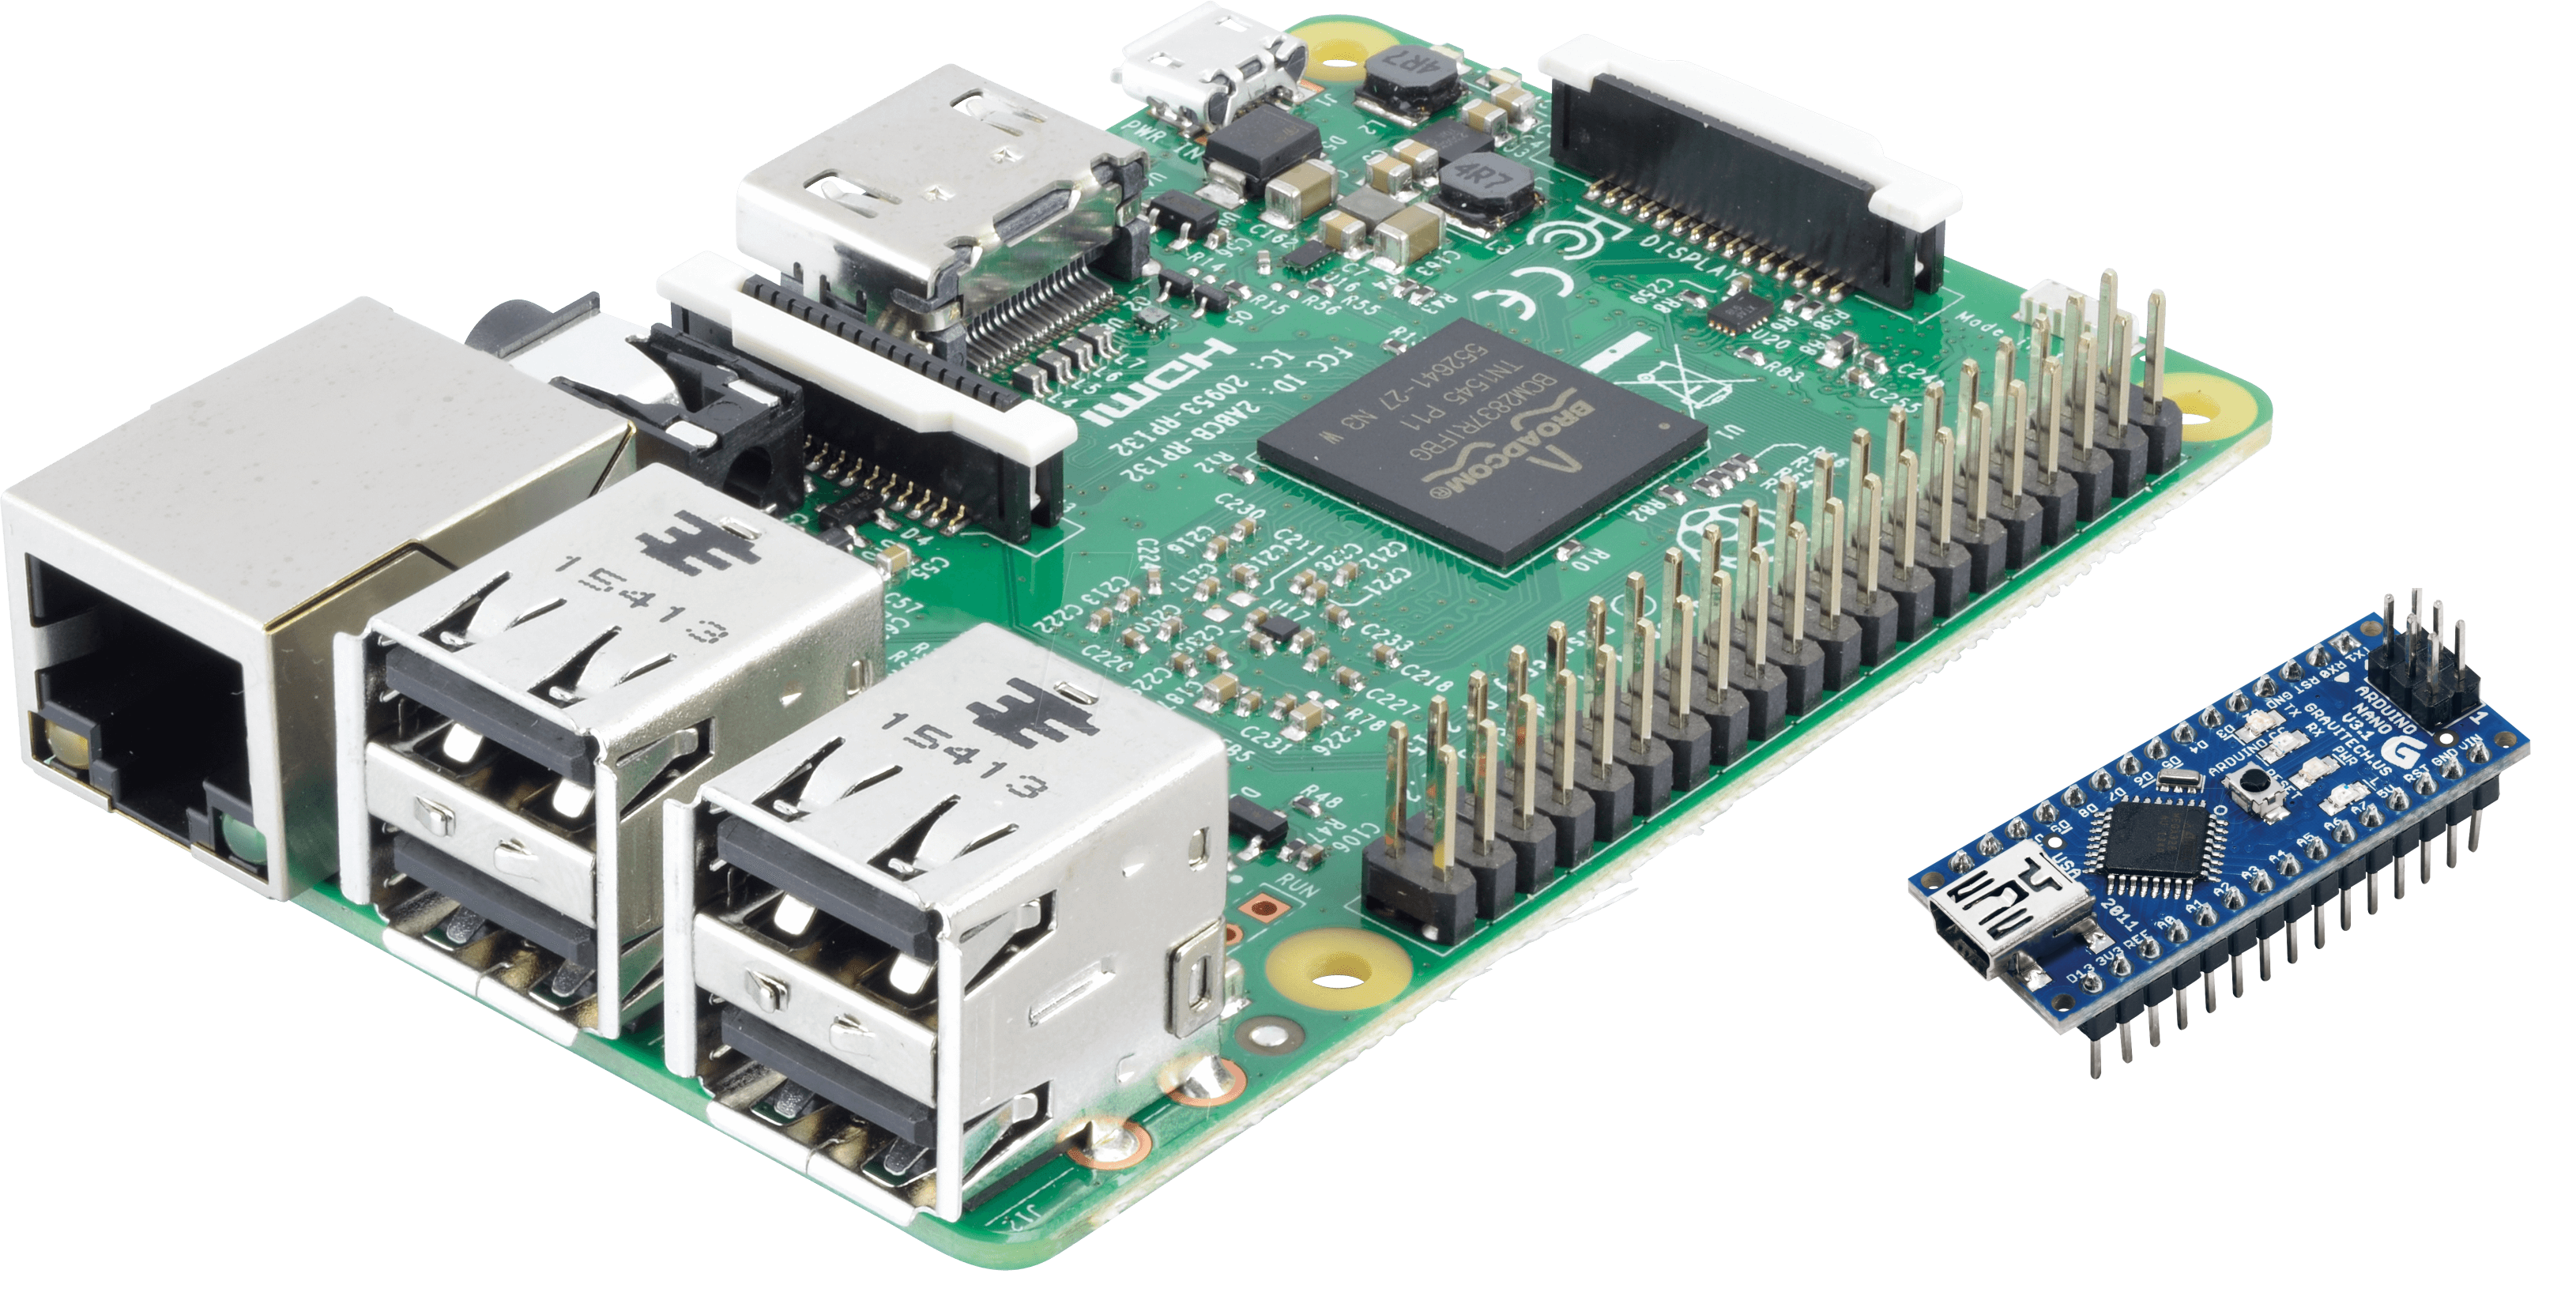
\includegraphics[width=0.7\textwidth]{img/raspArd}
	\caption{Raspberry y Arduino usados}
	\label{fig:RaspArd}
\end{figure}

Como anteriormente hemos comentado, el Arduino se encarga de las funciones de control de dirección y velocidad, a continuación mostraremos una imagen del conexionado completo, exceptuando el cable USB que une el Arduino y la Raspberry.

\begin{figure}[H]
	\centering
	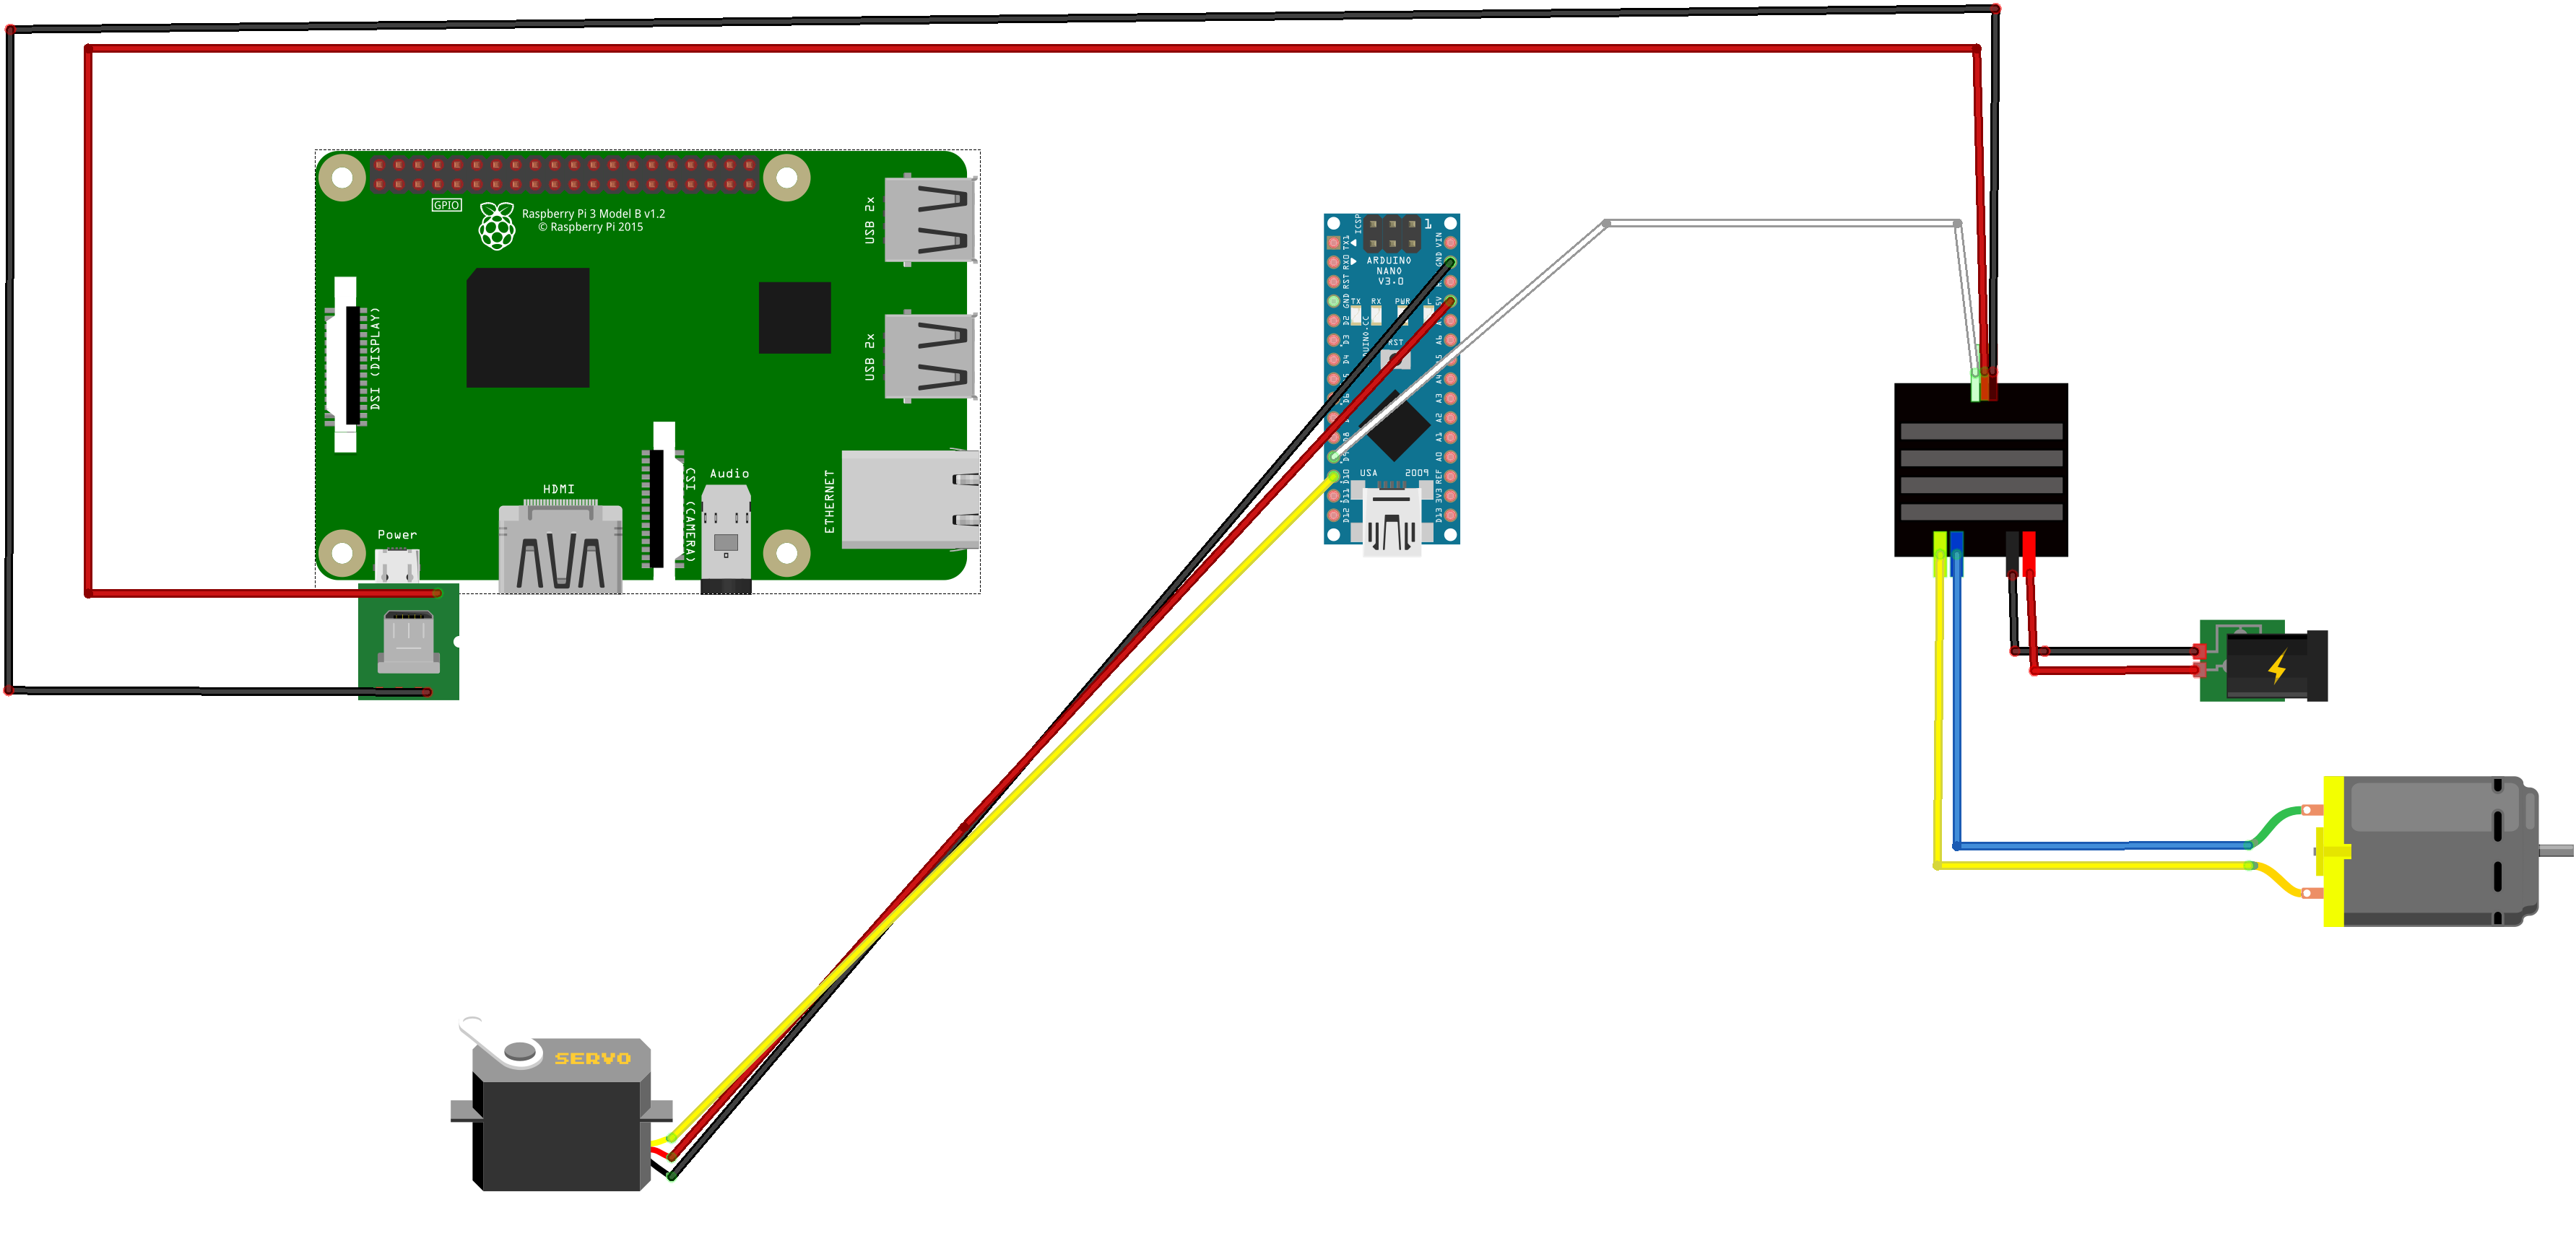
\includegraphics[width=0.9\textwidth]{img/conexionado}
	\caption{Conexionado}
	\label{fig:conexionado}
\end{figure}

Luego de las conexiones entre los distintos dispositivos, añadimos la webcam encargada de enviar las imágenes al sistema receptor. En este caso la webcam es una webcam USB normal utilizada en un PC cualquiera. Esta se conecta directamente a la Raspberry por el puerto USB. 

Para evitar tener tanta cantidad de cables, diseñamos e implementamos una PCB para integrar todas las conexiones y concentrarlo todo en una placa.

\begin{figure}[H]
	\centering
	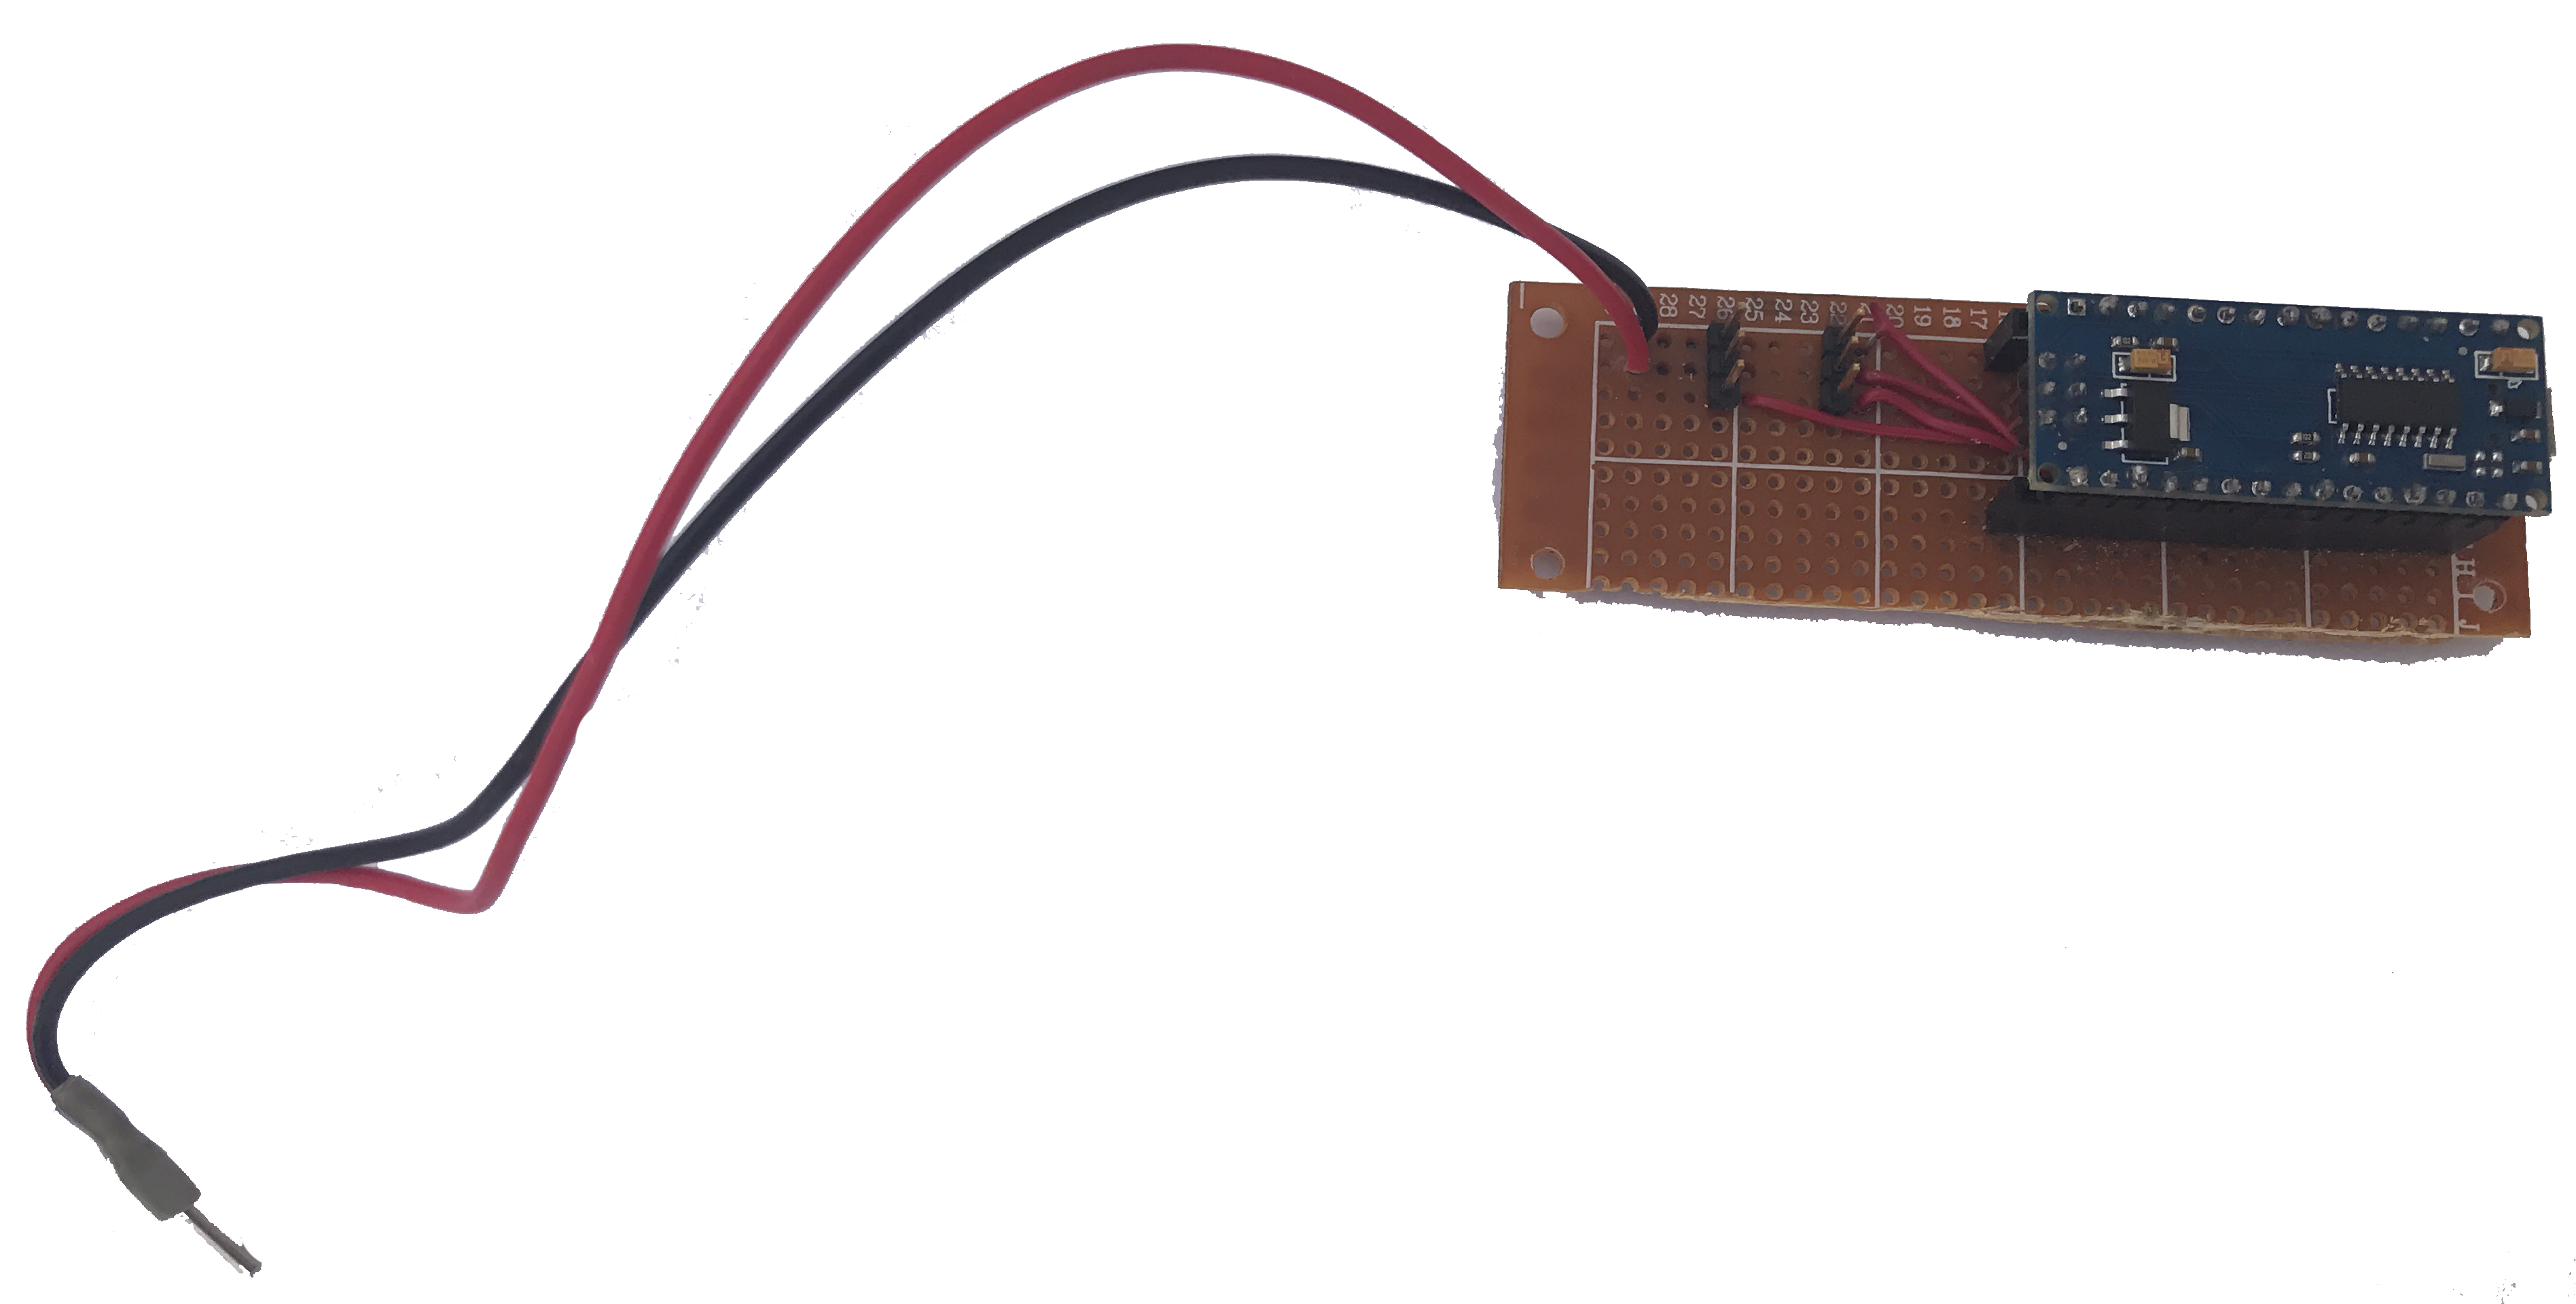
\includegraphics[width=0.7\textwidth]{img/pcb}
	\caption{PCB}
	\label{fig:pcb}
\end{figure}

En un momento determinado del proyecto, ya con las pruebas iniciadas, se detectó un pequeño problema. Este fallo era que al encender el coche, Raspberry y Arduino necesitan un tiempo prudencial para ponerse en marcha y que funcionen correctamente, pero a simple vista no se sabía cuando ocurría esto. Por tanto se decidió agregarle 3 LEDs de distintos colores, para saber en que estado se encuentra. Los LEDs son controlados por los puertos GPIO de la Raspberry, en concreto los pines 17, 23 y 24, además se le añadió a cada uno una resistencia para limitar el voltaje que cae en cada LED. El diseño del código de color fue el siguiente:

\begin{itemize}
	\item LED rojo: indica que el script Python se ha iniciado pero aún no se ha terminado la conexión con Arduino y la calibración de los dispositivos.
	\item LED verde: arroja que ya ha acabado el proceso de inicialización y está esperando una conexión entrante.
	\item LED azul: indica que hay una conexión establecida con el servicio de instrucciones (aclarar que el LED verde sigue encendido) y por lo tanto se supone que puede haber comunicación entre los pares.
	
\end{itemize}

La imagen que sigue muestra dichos LEDs y su emplazamiento.

\begin{figure}[H]
	\centering
	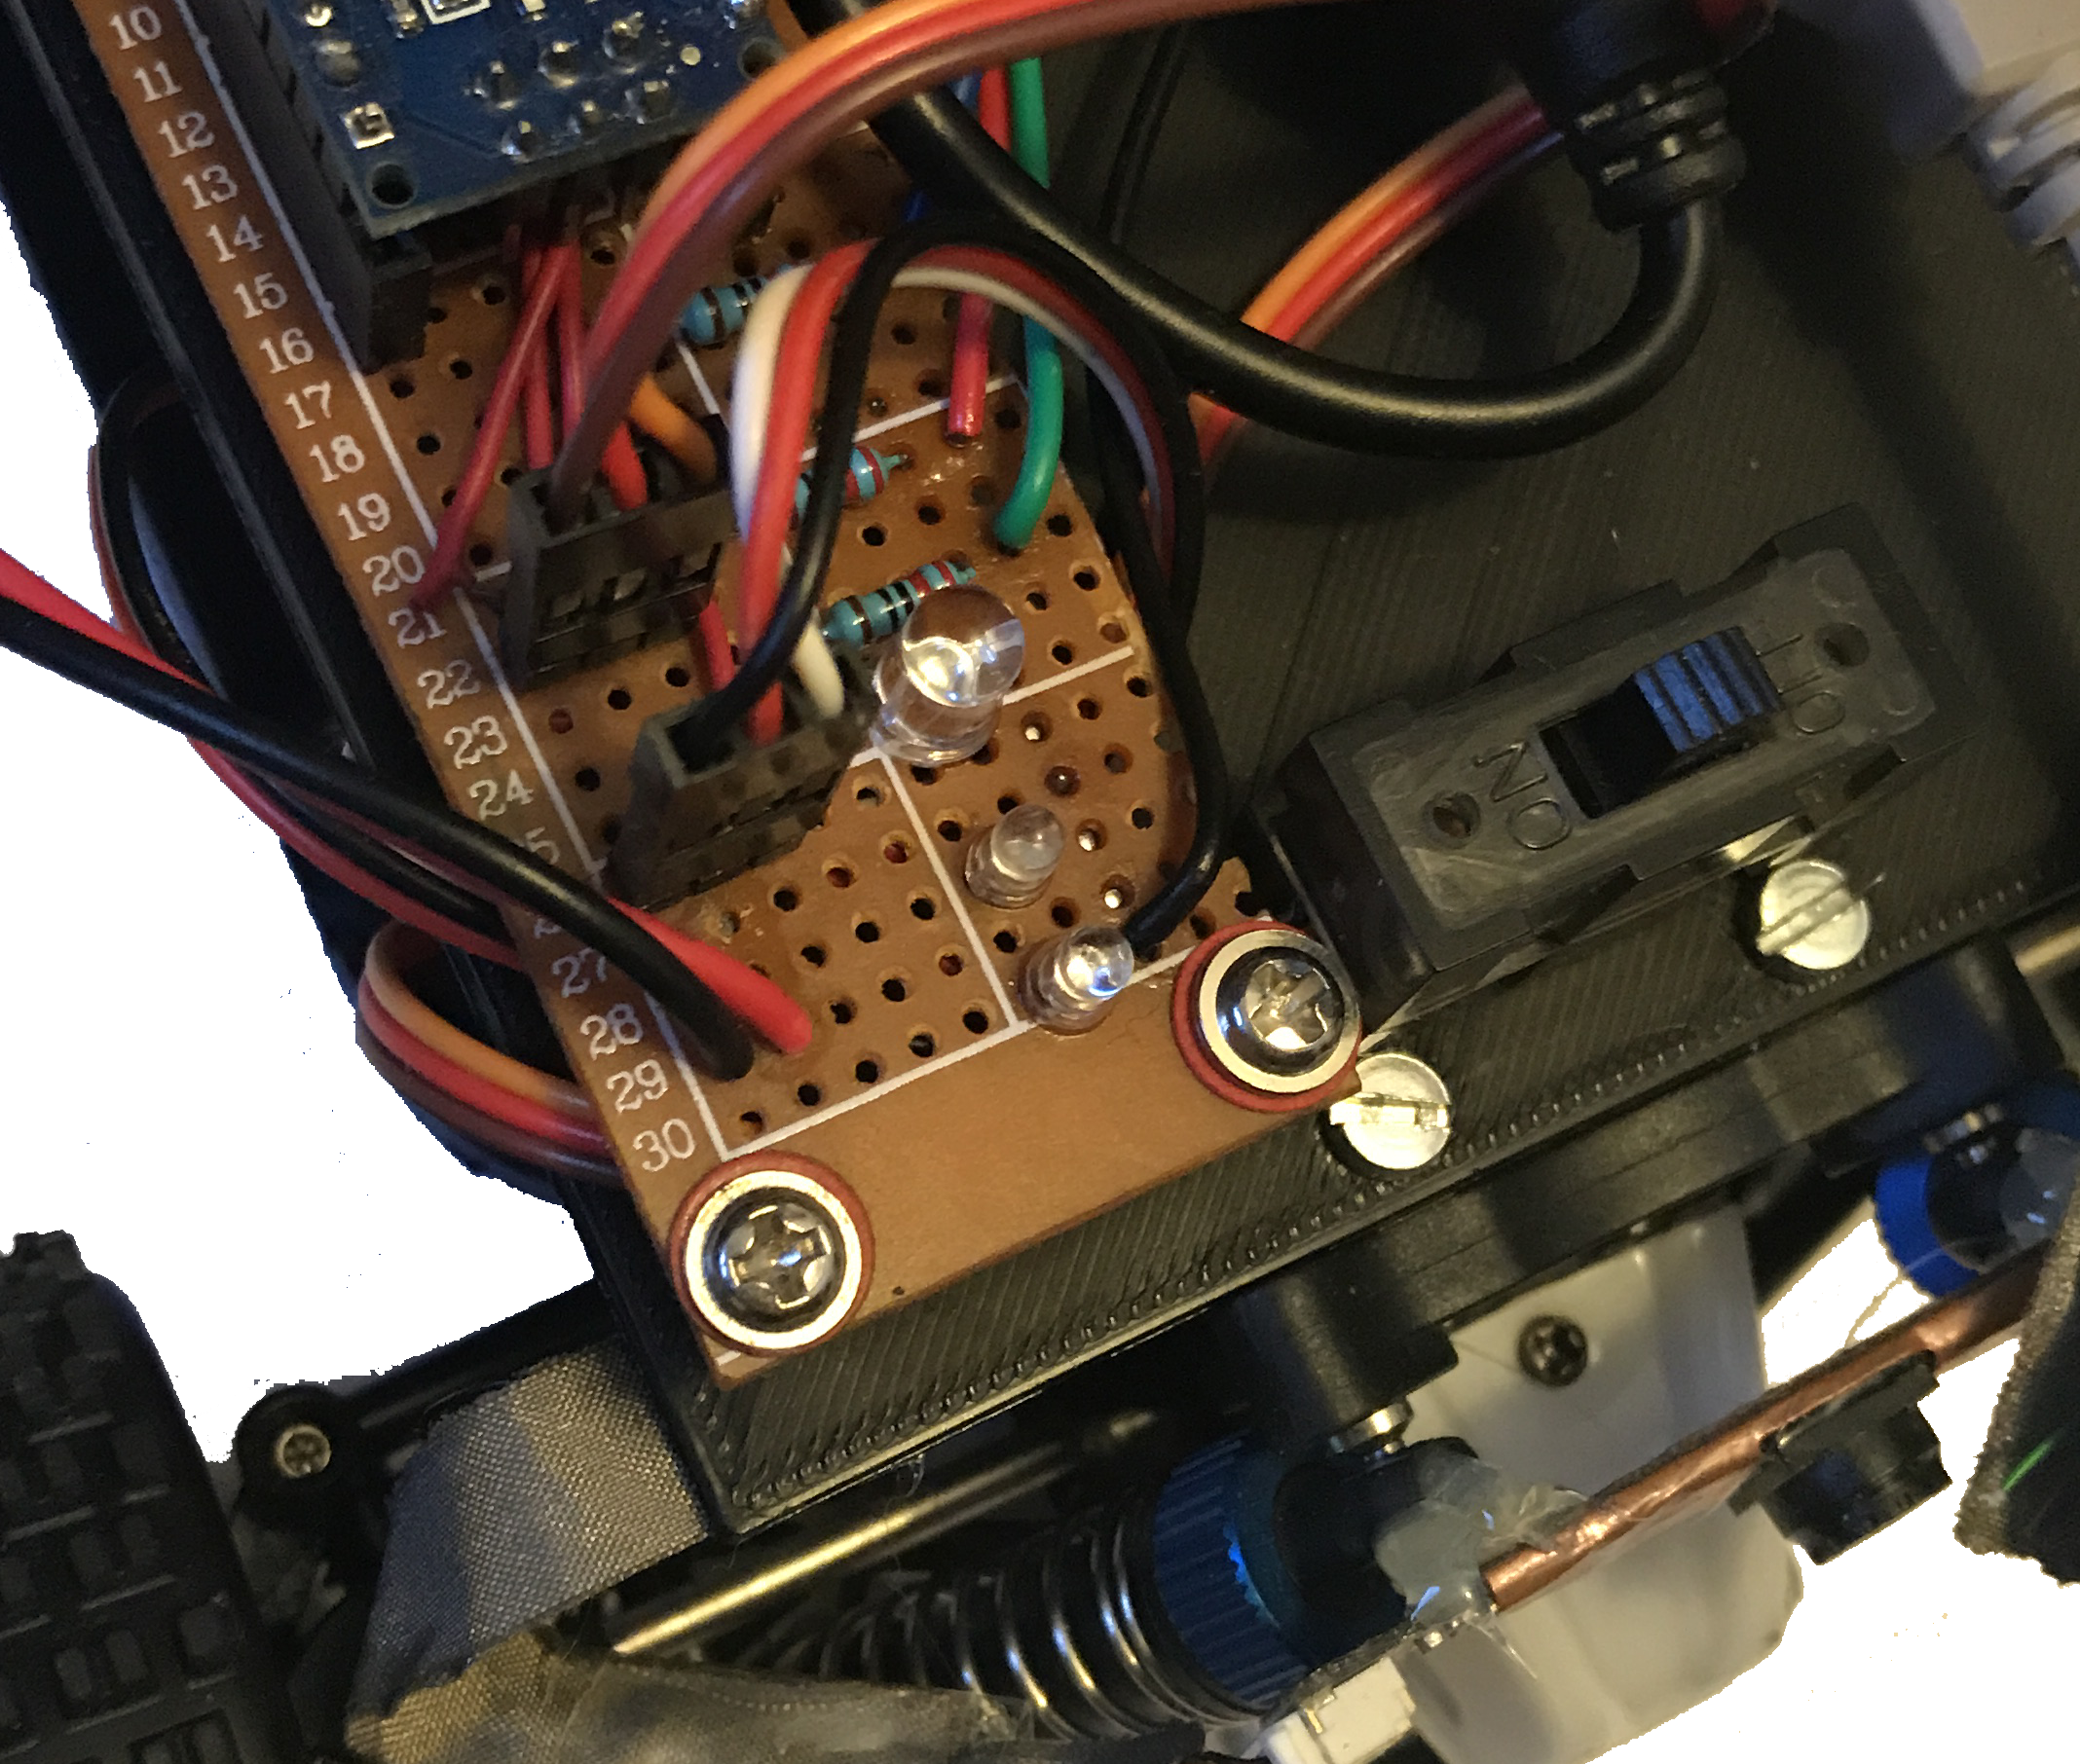
\includegraphics[width=0.7\textwidth]{img/leds}
	\caption{LEDs y su emplazamiento}
	\label{fig:leds}
\end{figure}



\begin{figure}[H]
	\centering
	\includegraphics[width=0.7\textwidth]{img/webCamAntigua}
	\caption{WebCam Antigua}
	\label{fig:webcamvieja}
\end{figure}

Después de hablar con una de las personas nombradas en los agradecimientos, llegamos a la conclusión de que esa cámara era demasiado grande y quedaba desorbitada en su emplazamiento. Después de investigar un poco, este cedió una WebCam integrada de un portátil, mucho más pequeña e integrable. Tras buscar el datasheet de dicha WebCam y usar ingeniería inversa, se procedió a soldar un cable USB. Con esto ya tenemos una WebCam mucho más pequeña, instalada como mostraremos a continuación.

\begin{figure}[H]
	\centering
	\includegraphics[width=0.7\textwidth]{img/webcamPortatil}
	\caption{WebCam portátil}
	\label{fig:webcamportatil}
\end{figure}

Llegados a este punto, se hizo necesario buscar la forma de compactar las placas dentro del coche. Para ello se diseñó una placa en la herramienta Tinkercad para ser impresa en 3D. Mostraremos a continuación una captura del diseño de la placa en dicha herramienta.

\begin{figure}[H]
	\centering
	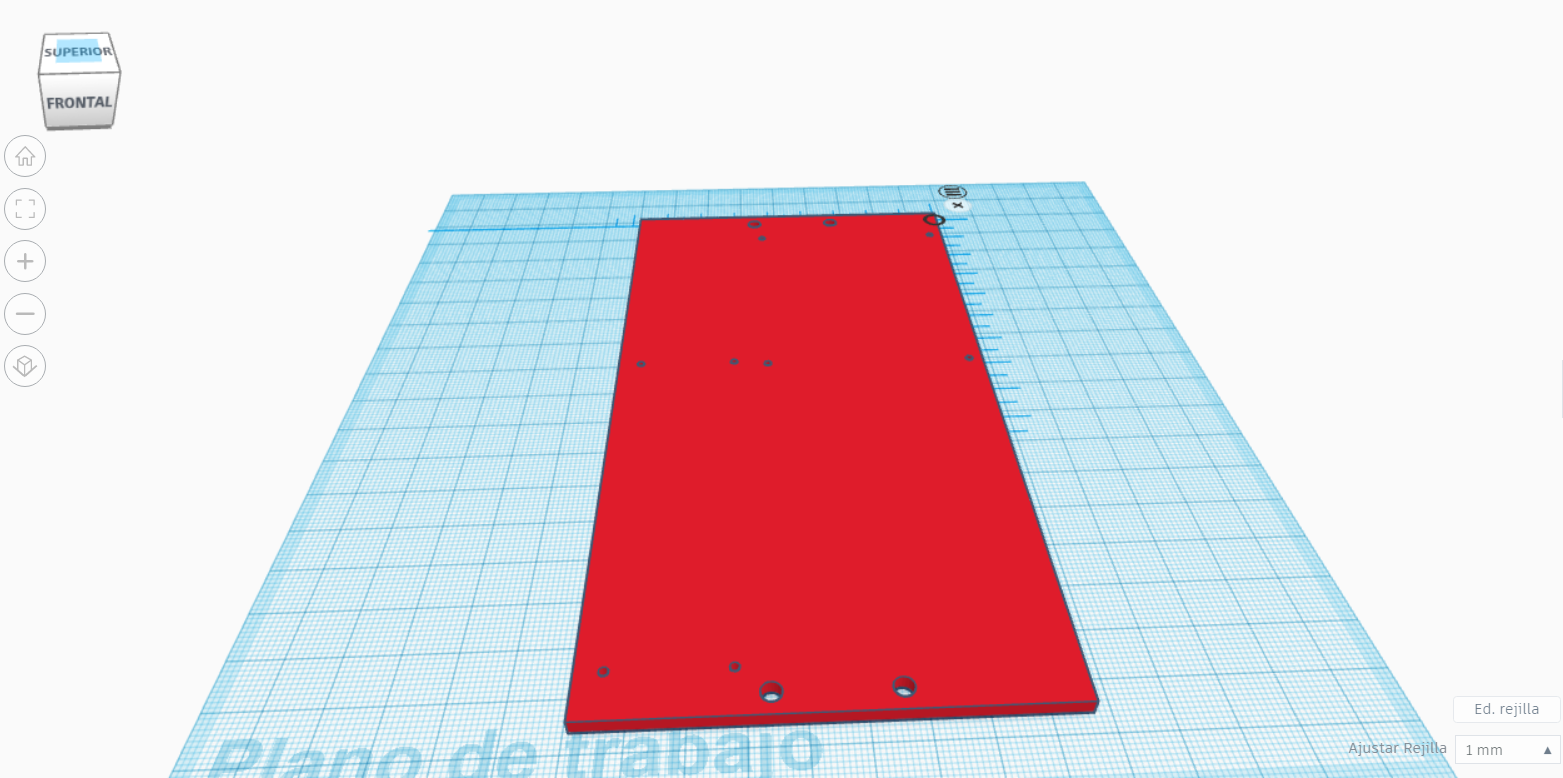
\includegraphics[width=0.9\textwidth]{img/soportePlacas}
	\caption{Placa diseñada 3D para el soporte de la Raspberrry y el Arduino}
	\label{fig:soporteplacas}
\end{figure}

A continuación vemos el resultado de dicho diseño, después de una hora de impresión.

\begin{figure}[H]
	\centering
	\includegraphics[width=0.5\textwidth]{img/soporteImpreso}
	\caption{Placa impresa en 3D}
	\label{fig:soporteplacasimpreso}
\end{figure}

Luego montamos la tornillería necesaria para atornillar la Raspberry Pi y el Arduino.

\begin{figure}[H]
	\centering
	\includegraphics[width=0.5\textwidth]{img/soporteImpresoTuercas}
	\caption{Placa impresa en 3D con la tornillería necesaria}
	\label{fig:soporteplacasimpresotuercas}
\end{figure}

Después de montar la tornillería, añadimos ambos dispositivos, tanto la Raspberry Pi como el Arduino.

\begin{figure}[H]
	\centering
	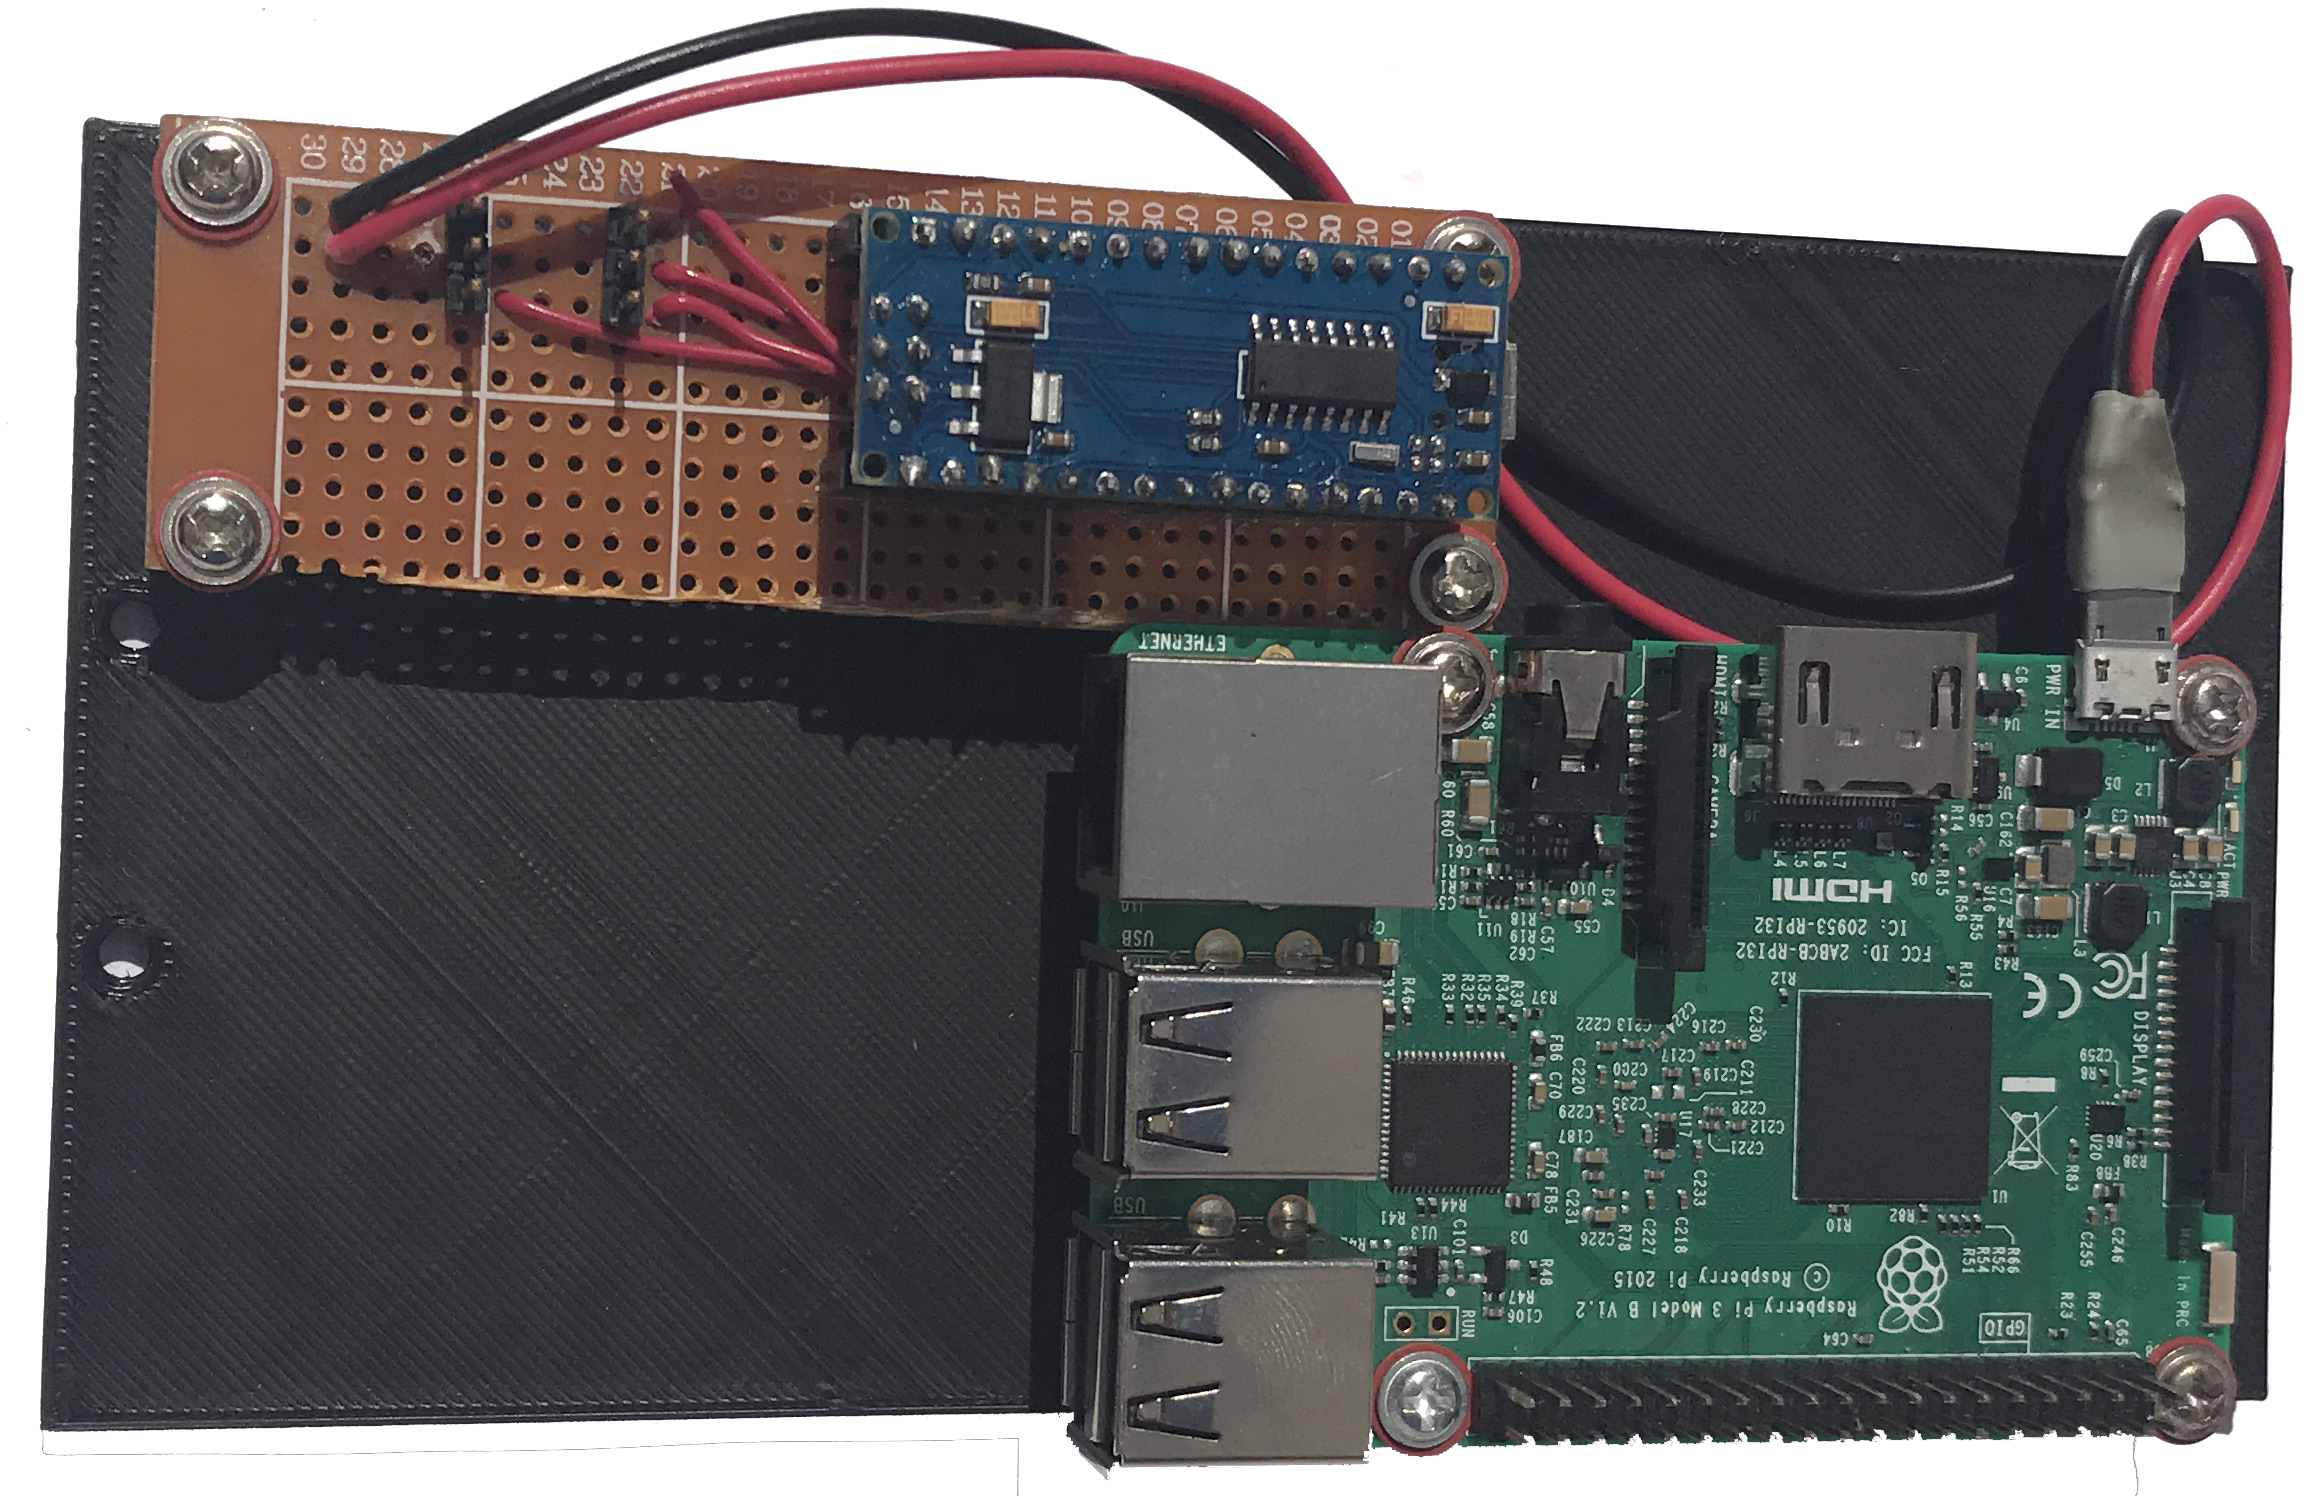
\includegraphics[width=0.7\textwidth]{img/soporteConPlacas}
	\caption{Placa impresa en 3D con los dispositivos montados}
	\label{fig:soporteconplacas}
\end{figure}

En la siguiente imagen mostramos como estaba el prototipo antes de utilizar dicha placa, con muchísimo desorden y con total imposibilidad de probar el prototipo de forma real, ya que cabía la posibilidad de que se desconectara alguna placa y/o hubiera algún daño en estas.

\begin{figure}[H]
	\centering
	\includegraphics[width=0.7\textwidth]{img/cocheConDesorden}
	\caption{Prototipo sin montar la placa de soporte}
	\label{fig:cochesinsoporte}
\end{figure}

A continuación, como la placa estaba diseñada para encajar perfectamente en el coche con cuatro tornillos de anclaje, procedimos a su montaje. Después de acoplar todo en el prototipo, placas, WebCam y cableado, quedó algo así, como resultado final.

\begin{figure}[H]
	\centering
	\includegraphics[angle=180,width=0.7\textwidth]{img/resultado}
	\caption{Prototipo resultante con todo montado}
	\label{fig:cochesResultante}
\end{figure}

\item Software


\begin{itemize}
	
	\item Sistema operativo
	
	Como plataforma software donde montar todo el sistema en la Raspberry hemos usado una distribución de Linux de Raspberry.org, Raspbian Jessie lite en concreto , la cual no tiene interfaz gráfica para evitar esa sobrecarga totalmente innecesaria.
	\medskip
	
	\item Conexión inalámbrica
	
	Se han utilizado dos programas para el correcto funcionamiento de la conexión.
	
		\begin{itemize}
			\item hostapd
			\smallskip
			
			Este software nos ha permitido configurar la Raspberry para que emita un SSID y cambiar las opciones de este, como puede ser nombre, contraseña, etc.
			\smallskip
			
			\item udhcpd
			\smallskip
			
			udhcpd simplemente es un servidor dhcp que dada la configuración que hemos introducido se encargará de que al conectar un dispositivo, este reciba una IP adecuada para que el sistema funcione.
			
		\end{itemize}
	\medskip
	\item Arduino
	
	En la parte del hardware comentamos la utilización de un Arduino para el control de dirección y tracción/freno. Para su integración, Raspberry y Arduino se comunican por USB, usándose comunicación serial. Se ha creado un pequeño protocolo de bienvenida entre ambos para asegurar el correcto funcionamiento de la conexión, que a continuación mostraremos.
	
	\begin{figure}[H]
		\centering
		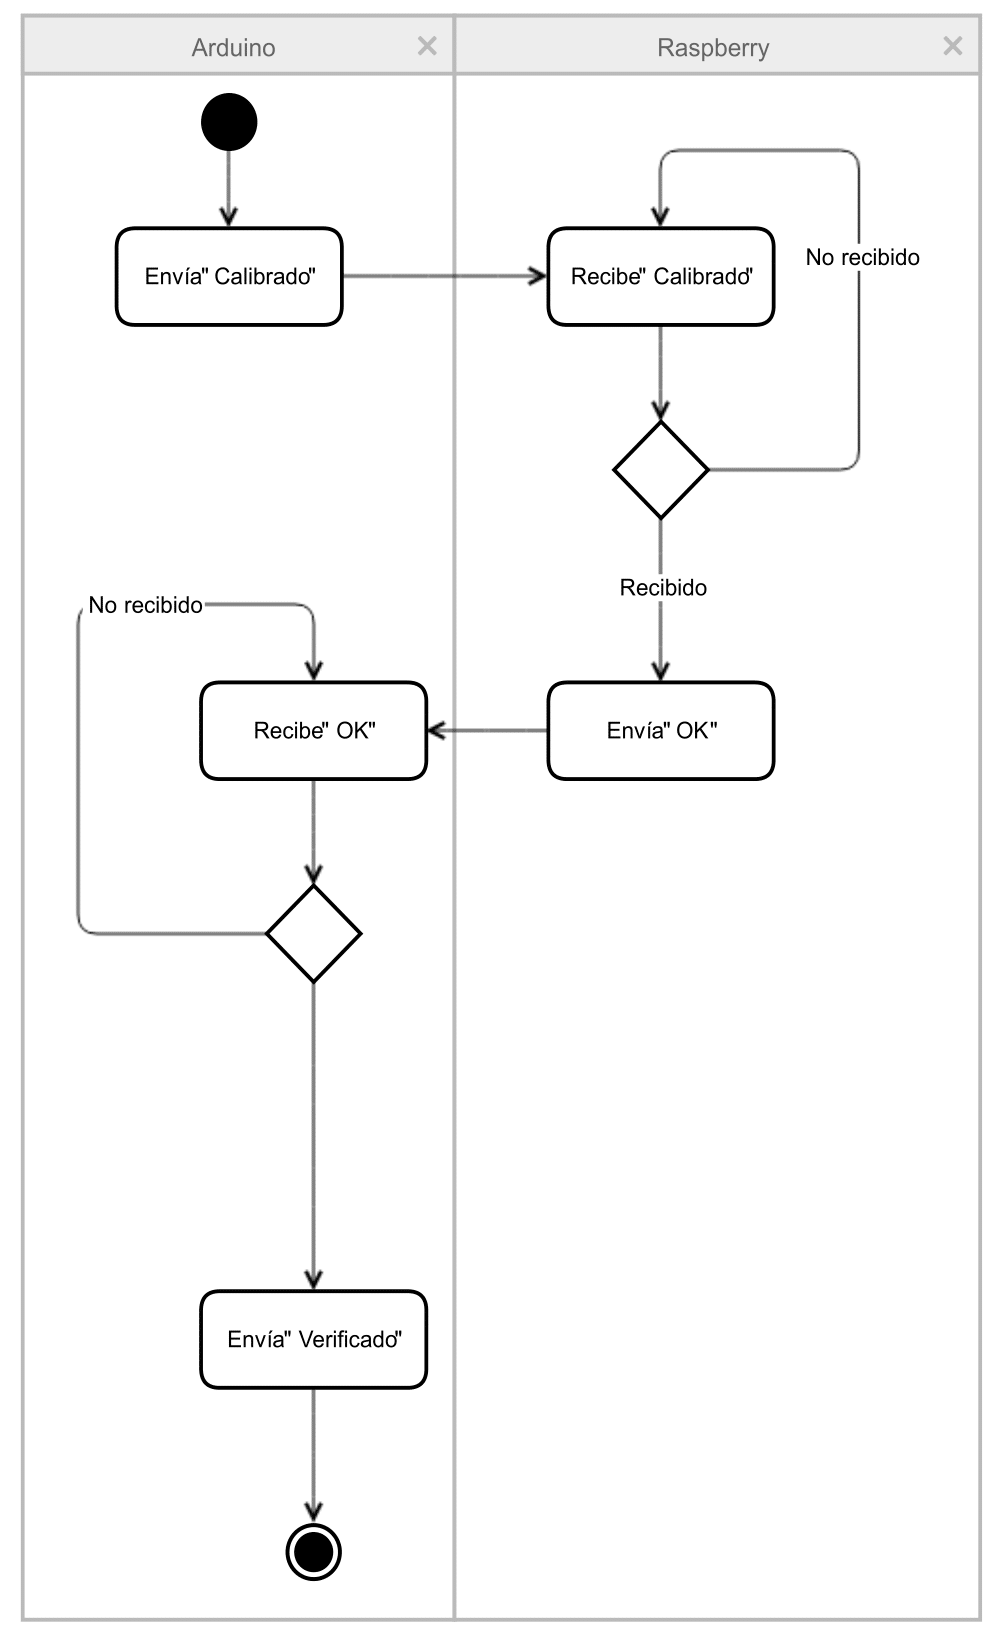
\includegraphics[width=0.7\textwidth]{img/umlComunicacion}
		\caption{UML de la verificación de la comunicación con Arduino}
		\label{fig:arduinoVerificacion}
	\end{figure}
	
	Además, se ha creado una codificación entendible por ambos extremos para mandar las instrucciones de lo que el coche debe realizar. Un ejemplo de instrucción sería <<$[$15,115$]$>> y su decodificación:
	\begin{itemize}
		\item $[$ : Carácter de comienzo de instrucción, esto se ha utilizado para reconocer que está comenzando una instrucción.
		\item Aceleración: 15\% 
		\item Dirección: 115º
		\item $]$ : Carácter de terminación de comando, esto se ha utilizado para reconocer el término de una instrucción.
	\end{itemize}
	
	Tras esta explicación cabe aclarar que la primera cifra antes de la coma indica el porcentaje de aceleración del vehículo comprendido entre -100 \% y 100 \%. En segundo lugar aparece la cifra que indica los grados de giro del servo, que teóricamente va desde 0º a 180º, pero que en nuestro caso está limitado a lo que nos deja girar la construcción del mecanismo de dirección que va desde los 65º hasta los 115º.
	

	El Arduino recibe dichas instrucciones y las decodifica como hemos descrito. Este respondiendo a una fórmula matemática que se intenta ajustar lo máximo al PWM que soporta el variador y la dirección, sus valores son modificados con una función que maneja los servos dependiendo de los grados a los que queramos posicionarlo y a la aceleración que deseemos imprimir.
	
	\begin{figure}[H]
		\centering
		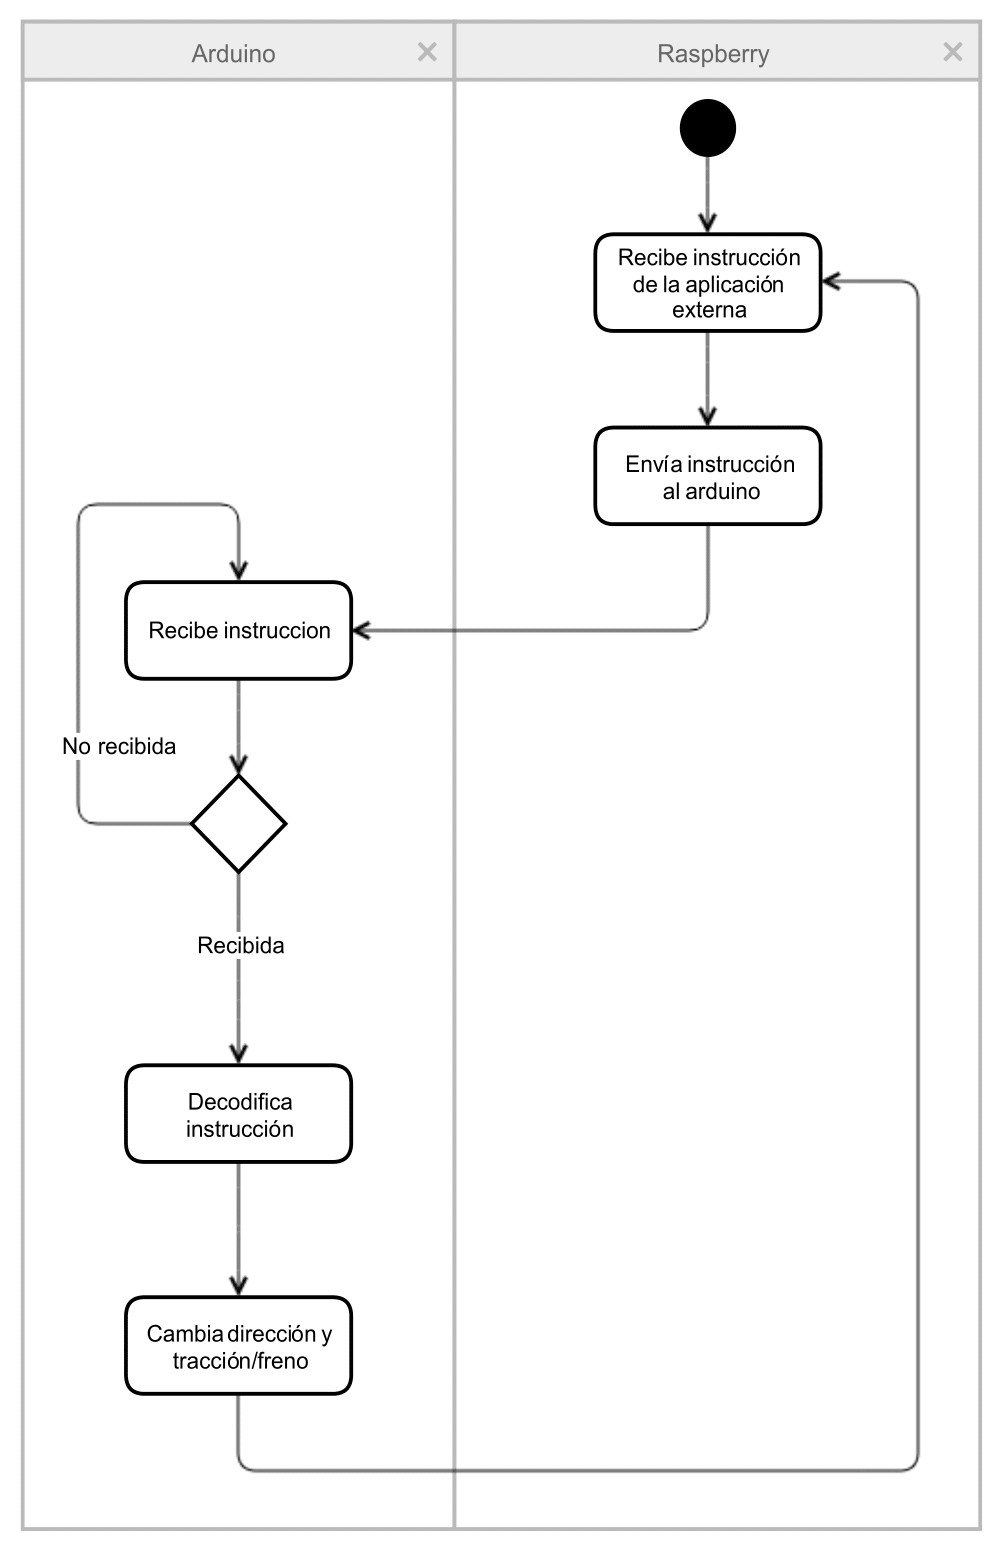
\includegraphics[width=0.7\textwidth]{img/umlCambio}
		\caption{UML de la comunicación del cambio de tracción/freno y dirección}
		\label{fig:arduinoCambios}
	\end{figure}
	
	Al conectar lo primero que el Arduino hace es calibrar tanto servo como variador a valores centrales, es decir, el servo a 90º que sería dirección recta, y el variador, mucho más importante porque necesita ser calibrado para su correcto funcionamiento, en un valor central de PWM que indica punto muerto. En este apartado hizo falta mucho tiempo ya que poniendo cualquier valor de PWM el variador no respondía, así que utilizando el método de ensayo y error descubrimos que primeramente hay que calibrarlo pasándole el valor de punto muerto.
	
	\medskip
	
	\item Servicio receptor de comandos
	
	Este es el hilo principal que vertebra a toda la aplicación, escrito en Python, en el cual primeramente se crea una variable de la clase Arduino, la cual se encarga de verificar internamente la correcta comunicación con este y tiene los métodos necesarios para el envío de comandos al Arduino Aquí el LED rojo esta activo, ya que nos indica que no se ha terminado el proceso de inicialización.
	
	En segundo lugar, lanzamos en segundo plano el servicio de streaming de vídeo (mjpg-streamer) que luego comentaremos. Lo hacemos utilizando una conexión a la consola de Linux mediante la clase os de python. 
	
	En tercer lugar, creamos el socket de la conexión de datos, la cual utilizaremos para el reconocimiento y procesado de las instrucciones. En este momento apagamos el led rojo y encendemos el verde, que indica que esta listo.
	
	Por último, la aplicación se quedará en bucle infinito esperando que alguien se conecte y si esto ocurre, espera datos de esa conexión hasta que el dispositivo que se ha conectado cierre el diálogo, además al conectarse un cliente, encendemos el LED azul para definir que estamos conectados con el cliente. Cada vez que recibe un dato lo procesa y ordena al Arduino que haga los cambios pertinentes. Las instrucciones tienen el mismo formato que las que se envían entre Raspberry y Arduino, con la salvedad de que se incluyen alguna más, como la instrucción ``close'' que sirve para cerrar explícitamente la conexión o la instrucción ``'' que también cierra la conexión y ha sido implementada porque Android al destruir la aplicación, si tiene una conexión activa, manda un paquete con datos vacíos. Cabe decir que la aplicación solo atenderá a una conexión, por simplicidad y porque se supone que solo se conecta un ``controlador'' por llamarlo de alguna manera, no tiene sentido que haya más de un dispositivo que lo controle conectado a la vez. 
	
	Al cerrar la conexión activa, el LED azul se apagará indicando que no hay ningún cliente conectado y el script volverá a esperar una nueva conexión entrante.
	
	También se tiene en cuenta la posible parada del script, para limpiar los puertos GPIO que usamos para los LEDs, ya que si no lo hacemos, al reiniciar el script corremos el riesgo de no poder usar dichos puertos.
	
	Al final de todo y tras llevar a cabo bastantes pruebas, decidimos convertir el script en un servicio que se inicie cuando encendemos la Raspberry sin necesidad de conectarnos a ella para iniciar dicho script.	\cite{servicio}
	
	\medskip
	
	\item Servicio streaming vídeo
	
	Para transmitir el vídeo en vivo hemos utilizado mjpg-streamer, un servicio de streaming de vídeo que consume pocos recursos, dado que estamos trabajando en la Raspberry, que nos limita mucho. Este además tiene internamente un servidor http para servir las imágenes o vídeos en directo. Esto facilitará mucho el consumo de las imágenes en una posible aplicación de escritorio o en la aplicación Android.
	
	\medskip
	
	\item Procesado de imágenes
	
		En este caso debido a la falta de tiempo, se descartó automatizar el prototipo con procesado de imágenes para solo implementar la detección de personas. La idea era insertar esta parte de código en la Raspberry pero tras probarlo se obtuvo un pésimo resultado en el procesado, ya que la cámara que usamos para el streaming de vídeo es la misma que queremos usar para este motivo. Dicha lentitud es debida a la imposibilidad de usar la cámara en exclusividad. Para ello, lo que se ha hecho es consumir las imágenes directamente del streaming, hecho que nos ralentiza en gran parte. Por contra, ganamos una buena característica y es la posibilidad de que sin modificar el script principal de la aplicación, podemos obtener el control procesando imágenes igualmente pero desde cualquier otro dispositivo, ya sea un PC o un dispositivo móvil.
		
		La manera más fácil que se nos ocurrió para no desaprovechar el trabajo dado la poca cantidad de tiempo disponible a estas alturas, fue procesar las imágenes desde un PC, con lo que ganaríamos en potencia de procesado. También se tuvo en cuenta el poder procesar las imágenes desde la misma aplicación Android ya diseñada, pero por facilidad y falta de tiempo, nos decantamos por la primera. Para ello hemos usado el mismo principio, descargar la imagen del streaming y procesarla luego. 
		
		Entrando en detalles del propio script, partimos de un script ya existente que detecta en una imagen a las personas que hay \cite{pedestrian}. Este se modificó en primera instancia para detectar personas en una continuidad de frames, en este caso capturados desde la propia WebCam del portátil. Acto seguido, tras la comprobación de que todo funcionaba perfectamente se pasó a buscar la manera de obtener las imágenes que la cámara del prototipo estaba captando. Como primera opción se probó intentar ocupar la cámara para este menester, pero al estar ya transmitiendo por streaming no era posible volverla a ocupar. Tras ello, se buscó la manera de obtener imágenes procedentes de un streaming mediante un script en Python y parseando las imágenes con openCV para que pudieran ser procesadas.
		
		En la imagen que sigue detallaremos con un diagrama de estados el funcionamiento de dicho programa.
		
		\begin{figure}[H]
			\centering
			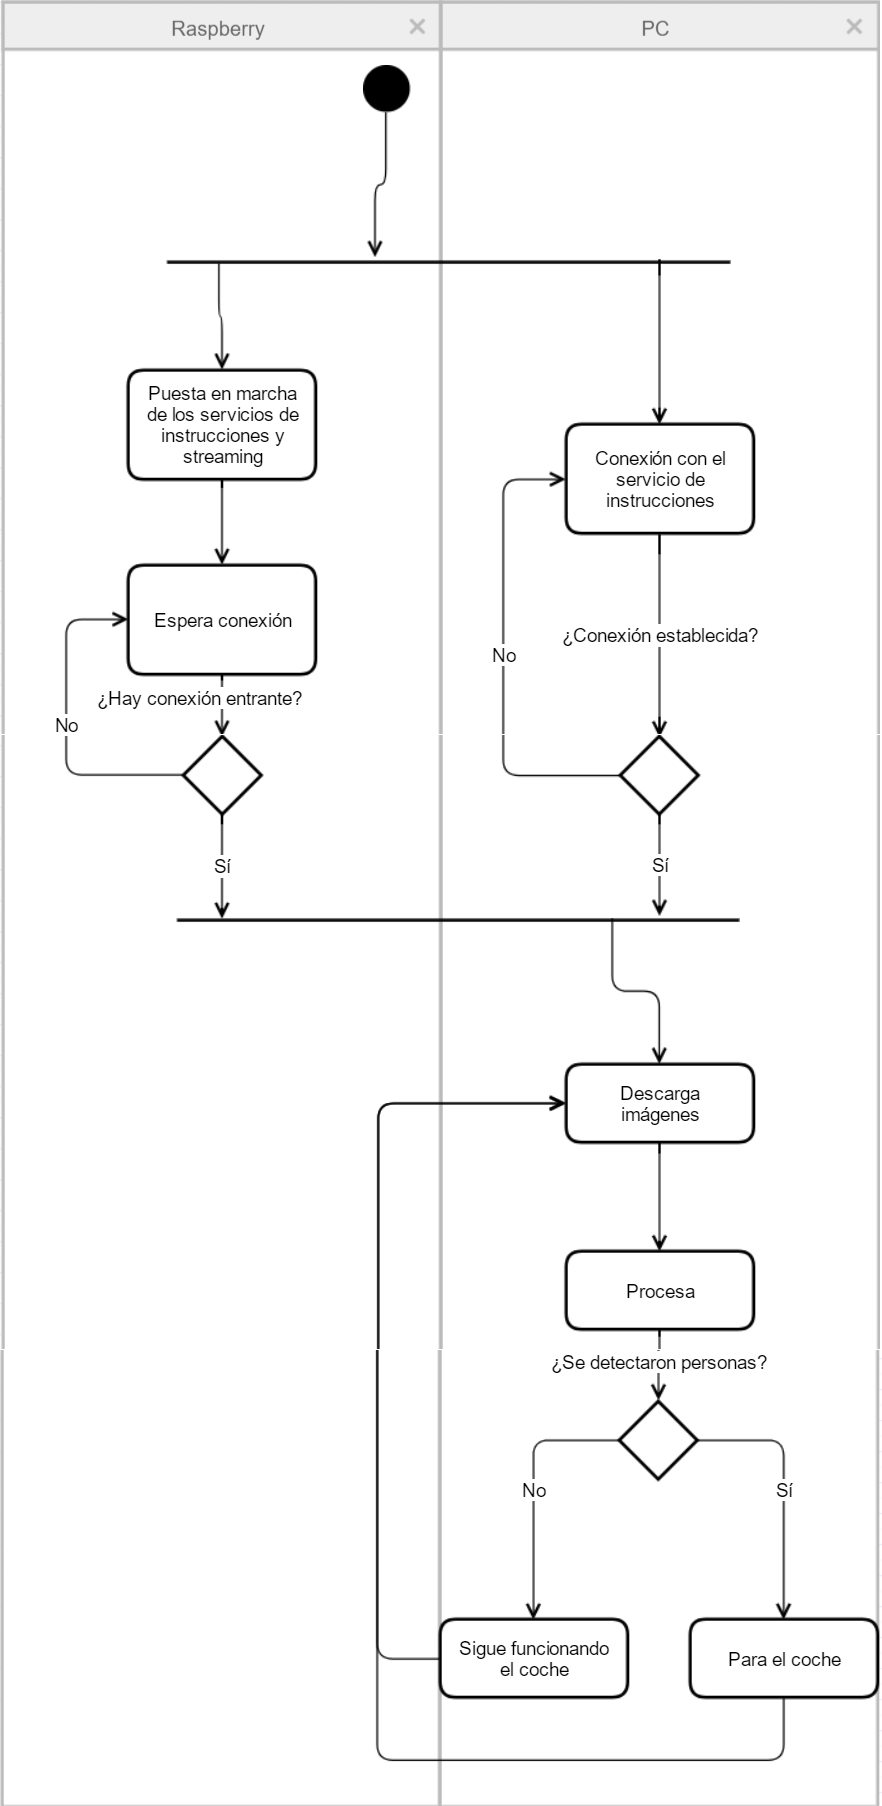
\includegraphics[width=0.7\textwidth]{img/procesadoUML}
			\caption{UML del procesado de imágenes}
			\label{fig:procesadoUML}
		\end{figure}
		
	
		\cite{OpenCV}

	\medskip

	\item Aplicación Android
	
	La aplicación Android esta basada en una app ya existente de código libre, obtenida de un repositorio en Bitbucket, llamada simpleMJPGView \cite{simpleMJPG}, que en principio, simplemente se dedica a consumir las imágenes que el coche emite con el protocolo MJPG. Tras obtener el código y añadirlo a Android Studio comenzamos las modificaciones necesarias para adaptarlo a nuestros requisitos. En primer lugar, se ejecutó la parte más importante de la aplicación, la conexión con el servicio de instrucciones del coche. Se tomó de referencia la IP que tenemos en las opciones de la aplicación. Tras ello la aplicación lanza un hilo en el que se hace una conexión TCP hacia el puerto 10000 de nuestra Raspberry Al conectar ya tenemos disponible el canal de comunicación de instrucciones. Luego se abre la conexión HTTP al puerto 8080 de nuestra Raspberry para obtener el stream de imágenes para representarlas en la aplicación. 
	
	Una vez todas las conexiones están activas se inicializa el acelerómetro para escuchar el sensor y mandar sus datos a la dirección del coche. Para evitar que el tráfico de instrucciones sea muy alto debido a las continuas lecturas del acelerómetro, se ha discretizado el valor de este a la parte entera, ya que así obviamos diferencias pequeñas de dirección y ruidos. Además solo se vuelve a mandar un comando si es distinto al anterior para evitar enviar varios comandos con el mismo valor. En cuanto al control de aceleración, ya sabemos que el prototipo tiene una velocidad alta, con lo que desde la aplicación solo permitimos el 50 \%  de la potencia disponible. Al igual que en la dirección hemos usado la misma táctica en cuanto a no repetir instrucciones ya enviadas. En el acelerador sí permitimos que el control actúe con toda su precisión porque da pasos de 1 unidad, algo asumible en cuanto a diferencia de aceleración y de tráfico generado.
	
	A continuación mostraremos unas capturas de la aplicación ejecutada en una tablet Samsung Galaxy Tab 3 7":
	
	\begin{figure}[H]
		\centering
		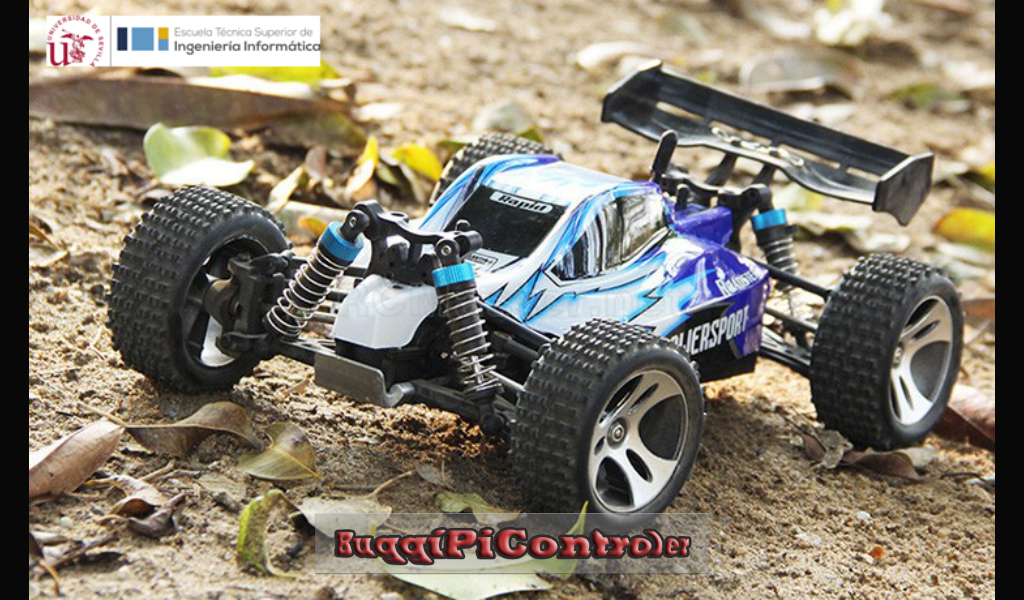
\includegraphics[width=0.7\textwidth]{img/inicio}
		\caption{Captura de la pantalla de inicio de la aplicación}
		\label{fig:capturaInicio}
	\end{figure}

	\begin{figure}[H]
		\centering
		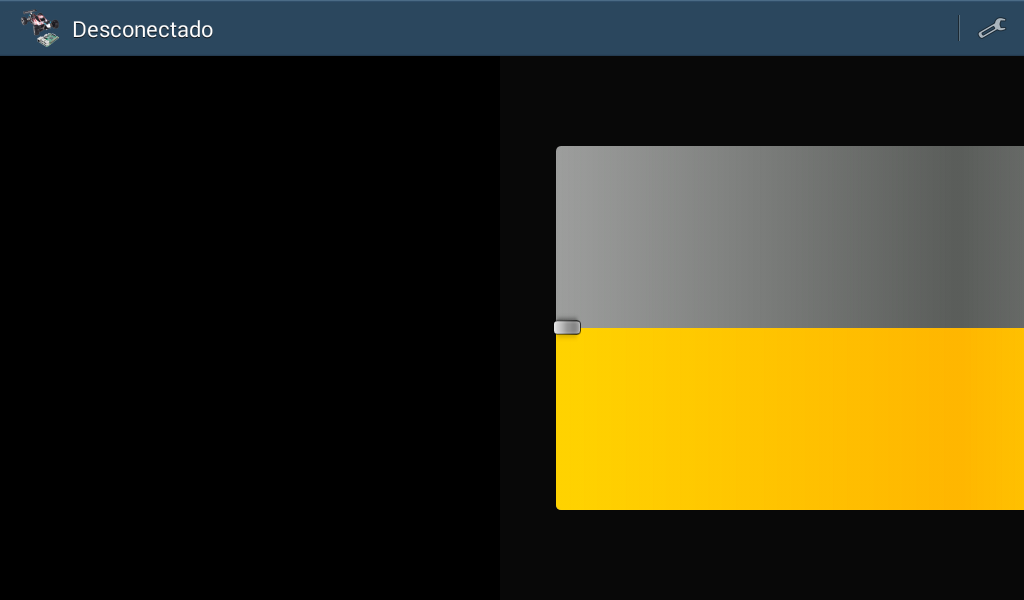
\includegraphics[width=0.7\textwidth]{img/sin_conexion}
		\caption{Captura de la pantalla principal de la aplicación sin conexión}
		\label{fig:capturaSinConexion}
	\end{figure}

	\begin{figure}[H]
		\centering
		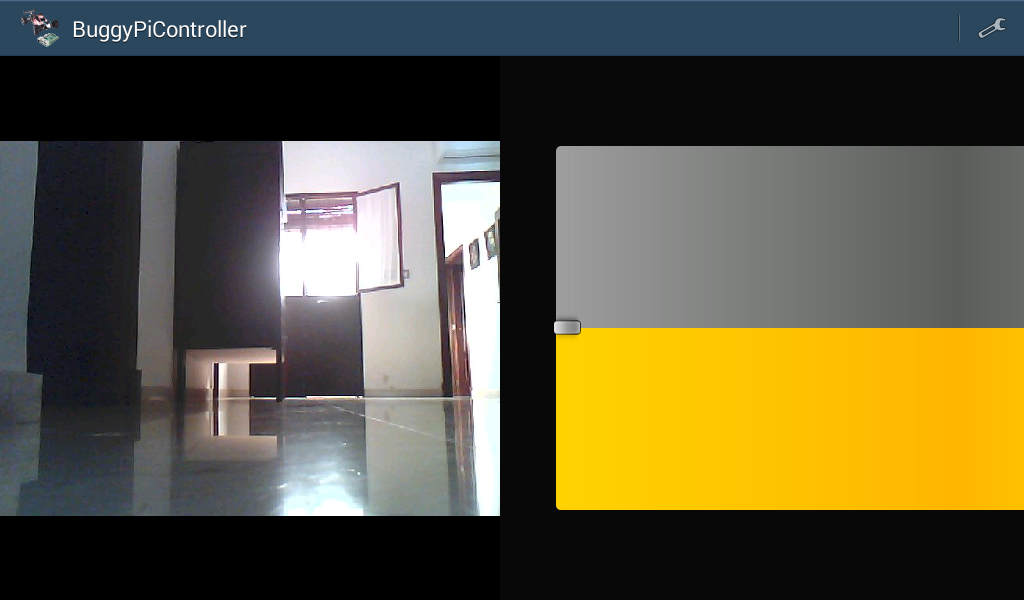
\includegraphics[width=0.7\textwidth]{img/conectado}
		\caption{Captura de la pantalla principal de la aplicación funcionando}
		\label{fig:capturaConConexion}
	\end{figure}
	
	\begin{figure}[H]
		\centering
		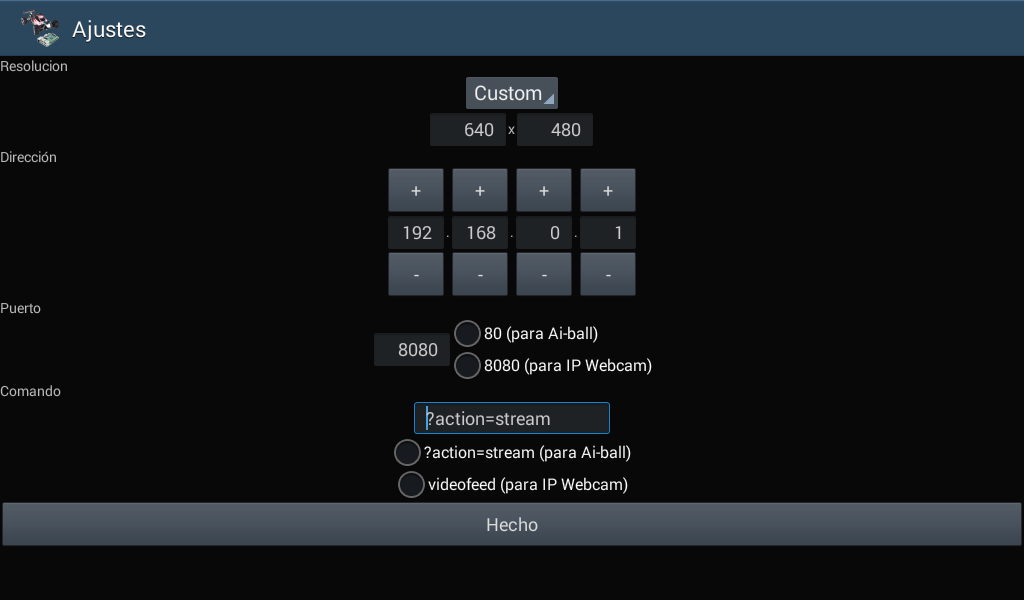
\includegraphics[width=0.7\textwidth]{img/opciones}
		\caption{Captura de la pantalla de opciones de la aplicación}
		\label{fig:capturaOpciones}
	\end{figure}
	
	
	\medskip
	
\end{itemize}
\end{itemize}


\section{Pruebas del sistema} 

Las pruebas realizadas del sistema han sido muy diversas, ya que en cada paso del diseño del software y hardware correspondiente se han sucedido todo tipo de test por partes para cerciorar el correcto funcionamiento de las modificaciones. A continuación pasaremos a describir las más importantes:

\begin{itemize}
	\item Arduino:
	
		Las primeras pruebas que se realizaron en el proyecto fueron bastante simples y se hicieron en esta parte del proyecto. Se empezó simplemente probando el control de servo y variador, una simple prueba de como responden estos ante el control del Arduino. Esta se realizó lanzando unas instrucciones concisas y prefijadas para comprobar el correcto funcionamiento de las piezas descritas.
		
		Después de comprobar que todo era posible y funcionaba correctamente se realizó el software en Arduino que recibía las instrucciones, este las decodificaba y actuaba en consecuencia. En este paso, para verificar el correcto funcionamiento, conectábamos el Arduino al puerto USB del PC y desde el IDE de Arduino entrabamos al monitor del puerto serie. A continuación mandábamos los comandos pertinentes para ejecutar el protocolo de bienvenida perfectamente. En cuanto estaba preparado para recibir instrucciones se lanzaba una serie de órdenes predefinidas y con ciertos errores, para cerciorar que en todo momento realizaba lo que esperábamos. 
		
	\item Raspberry:
	
		Antes de empezar con el servidor que debe ser el principal servicio que preste la Raspberry, había que configurar el wifi. Para ello, utilizamos otra microSd para no modificar el sistema donde se estaba desarrollando. En esta nueva microSd se realizaron las pruebas pertinentes para las configuraciones deseadas de la conexión wifi y por ende, la del servidor dhcp.
	
		En cuanto al sistema Python implementado en la Raspberry hay dos claras pruebas que se han realizado.
		
		En primer lugar se implementó la conexión por USB con el Arduino. Con lo cual se lanzaron una serie de pruebas en las cuales se enviaban una batería de comandos desde el código Python por serial al Arduino y que este respondiera tal cual se esperaba de él.
		
		Como segunda prueba, se comprobó la parte de la conexión para las instrucciones. En este caso, primeramente se hizo un cliente también en Python que se conectara al servicio, para verificar la correcta recepción de los comandos. Luego ya se hizo la misma prueba pero ya conectando desde una primera versión de la aplicación Android.
		
		Como última prueba, se unió el servicio de escucha de instrucciones y la conexión con el Arduino. Ya una vez unido, se volvieron a repetir las pruebas anteriores. Desde un script Python se le enviaba una batería de instrucciones y solo cabía esperar que el coche hiciera las indicaciones. Tras el éxito, se hizo lo mismo pero desde Android, con una primera versión de la aplicación Android.
		
	
	
	\item Webcam:
	
		Igual que en el apartado anterior, usamos la microSd de pruebas para probar los distintos sistemas de streamer. Se probaron un script Python con openCV para la obtención de imágenes, que fue descartado por el alto consumo de recursos. Luego se hicieron todas las pruebas con el streamer ahora utilizado, MJPEG-Streamer. En este se probó en primera instancia tomar imágenes e irlas guardando en un directorio pero también era bastante pesado. Así que la última configuración fue la más acertada. Este streamer tiene la opción de emitir directamente a un servidor HTTP. Con esto lo lanzamos y comprobamos desde cualquier navegador cual era el resultado y si la velocidad de transmisión era aceptable.
		
		Luego ya integrado con el script principal de los servicios, probamos la aplicación SimpleMJPEG de Android, para consumir las imágenes y comprobar si era fluida las imágenes.
	
	\item Aplicación Android:
	
		Como anteriormente comentamos la aplicación se ha probado en dos partes. En primer lugar la parte de sensor de aceleración de la tablet y el slider, todo ello con la conexión de instrucciones. Para ello se usó una aplicación con solo esta parte y se usó durante unos 20 min para comprobar la respuesta del vehículo.
		
		En segundo lugar se comprobó la parte del consumo de imágenes. Para ello solo hubo que encender el servicio y hacer unas pruebas de si las imágenes se recibían y si es aceptable el flujo que nos ofrece.
		
		Por último se completó la aplicación y con ambas partes y se puso a prueba si había demasiado retardo al añadir ambas cosas al canal de la comunicación.
		
	\item Procesado de imágenes:
	
		En primer lugar se probó a descargar desde un script en Python los frames que produce el streaming de vídeo del coche. Para ello se descargó y luego se mostró en una pantalla dichos frames.
		
		A continuación se probó la detección de personas desde la WebCam del ordenador para ajustar los valores de la función que detecta las personas. Tras prueba y error con dichos valores, sopesando entre rendimiento y precisión, integramos la descarga de imágenes con la detección de personas. Entonces probamos como era el rendimiento del conjunto.
		
		Al comprobar todo lo anterior, se prosiguió con la siguiente prueba, la integración del control del coche con la detección de personas. Después de programar todo lo necesario, se tuvo en pruebas unos 15 min, intercalando varias personas en la imagen y nadie, para ver si el resultado es el esperado. Y así fue, solo que con un poco de retardo, pero acabó funcionando perfectamente. 		
		
		
	
	\item Funcionamiento completo:
	
		Con todas las pruebas anteriormente comentadas, estaba más que suficientemente probado todo, ya que se ha ido probando parte por parte la integración. Aún así se acometieron algunas pruebas no realizadas antes, como por ejemplo, al integrar el script como un servicio de Linux, había que probar si funcionaba cada vez que arrancaba sin hacer nada.
		
		Además se probó que no se pudieran conectar más de un cliente a la vez. Al trastear con esta prueba se halló un problema con los puertos de entrada/salida que controlan los LEDs, que al terminar una conexión limpiaba estos. El problema radicaba justo cuando se cerraba la primera conexión, se tomaron las medidas oportunas y se arregló el problema.
		
		También hubo que modificar que al cerrar el programa se limpiaran los puertos de entrada/salida, ya que si hay algún problema y el script se reinicia sin limpiarlos, nos dará un error y no podrá continuar, así que se hizo esa prueba y al principio falló, con lo que se modificó.
		
		A continuación se probó en general todo el proyecto, así como el tiempo de respuesta, alcance y rendimiento.	
		
	
\end{itemize}


\chapter{BLOQUE 3: PLANIFICACIÓN DEL PROYECTO}
\section{Planificación temporal inicial} 
A continuación detallaremos una planificación temporal a priori:

\begin{figure}[H]
  \centering
    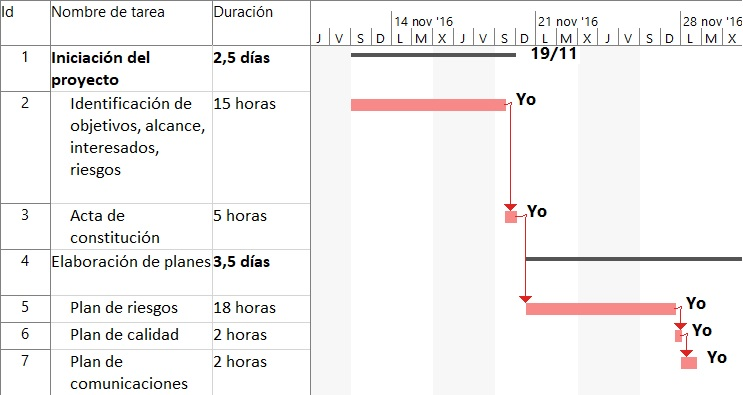
\includegraphics[angle=270,width=0.5\textwidth]{img/ganttInicial}
  \caption{Diagrama de Gantt Inicial}
  \label{fig:ganttInicial}
\end{figure}

\begin{figure}[H]
	\centering
	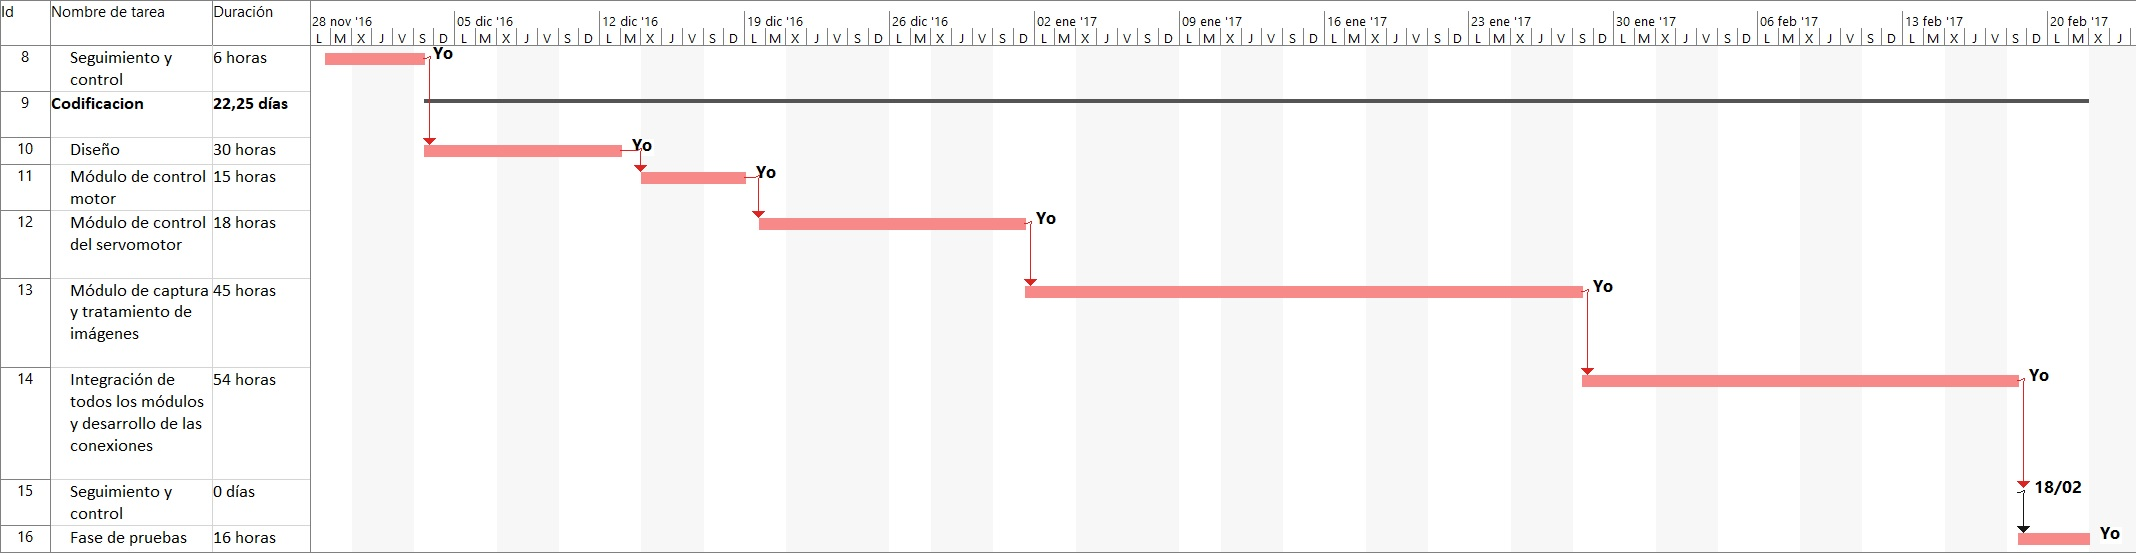
\includegraphics[angle=270,width=0.45\textwidth]{img/ganttInicial_2}
	\caption{Diagrama de Gantt Inicial 2}
	\label{fig:ganttInicial2}
\end{figure}

\begin{figure}[H]
	\centering
	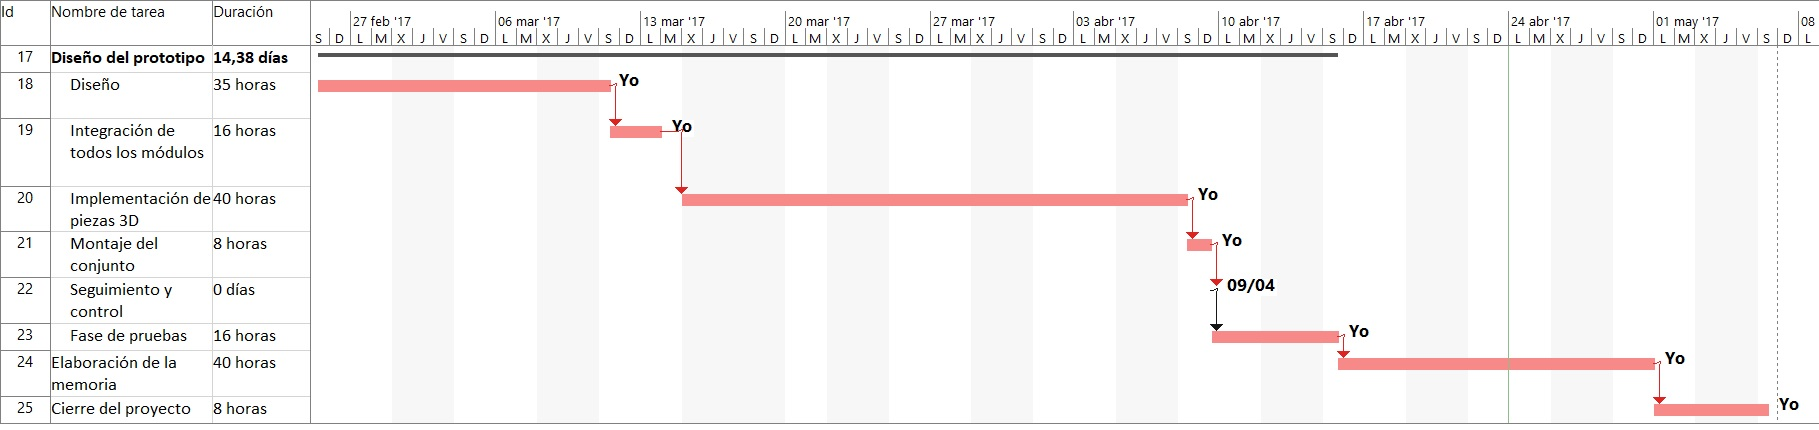
\includegraphics[angle=270,width=0.40\textwidth]{img/ganttInicial_3}
	\caption{Diagrama de Gantt Inicial 3}
	\label{fig:ganttInicial3}
\end{figure}



\section{Planificación financiera inicial} 
A continuación detallaremos una planificación financiera a priori:
\begin{itemize}
    \item Modelo a escala de un buggy: 43,85 \euro
    \item Raspberry Pi 3 modelo B: 38,70 \euro
    \item Variador (control motor): 9,45 \euro
    \item Clavijas conexión motor: 0,35 \euro
    \item Clavija conexión batería: 1,20 \euro
    \item Webcam: 15 \euro
    \item Cables interconexión: 2 \euro
    \item Horas de trabajo: 389 h * 8 \euro/h = 3112 \euro

\fbox{ Presupuesto total: 3222,55 \euro}
\end{itemize}

\section{Planificación temporal final (real)}

\begin{figure}[H]
	\centering
	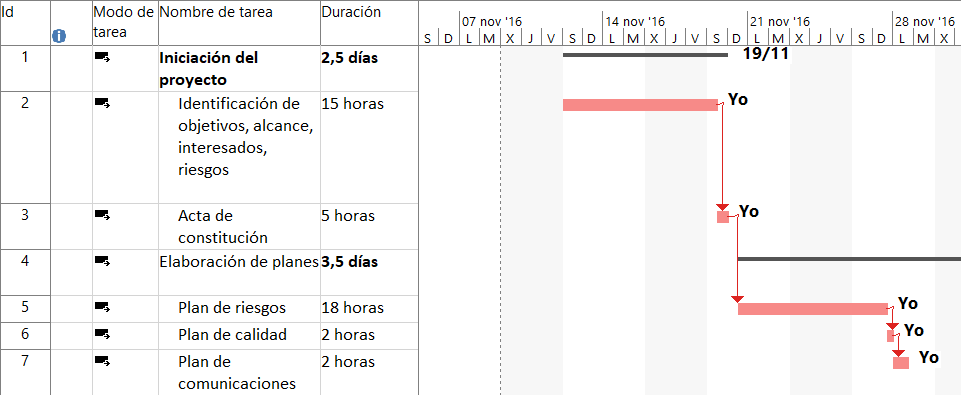
\includegraphics[angle=270,width=0.5\textwidth]{img/ganttFinal}
	\caption{Diagrama de Gantt Final}
	\label{fig:ganttFinal}
\end{figure} 

\begin{figure}[H]
	\centering
	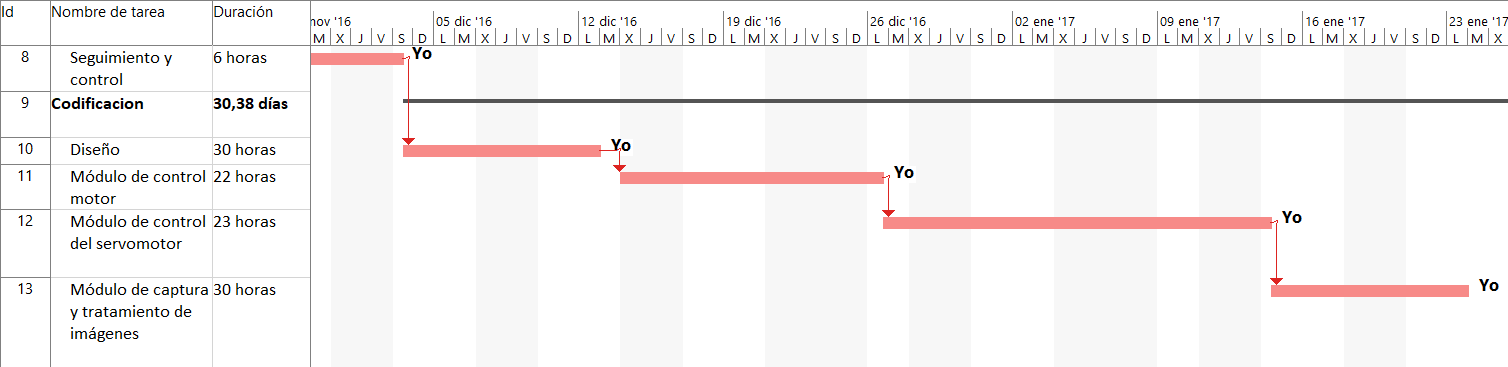
\includegraphics[angle=270,width=0.4\textwidth]{img/ganttFinal2}
	\caption{Diagrama de Gantt Final 2}
	\label{fig:ganttFinal2}
\end{figure}

\begin{figure}[H]
	\centering
	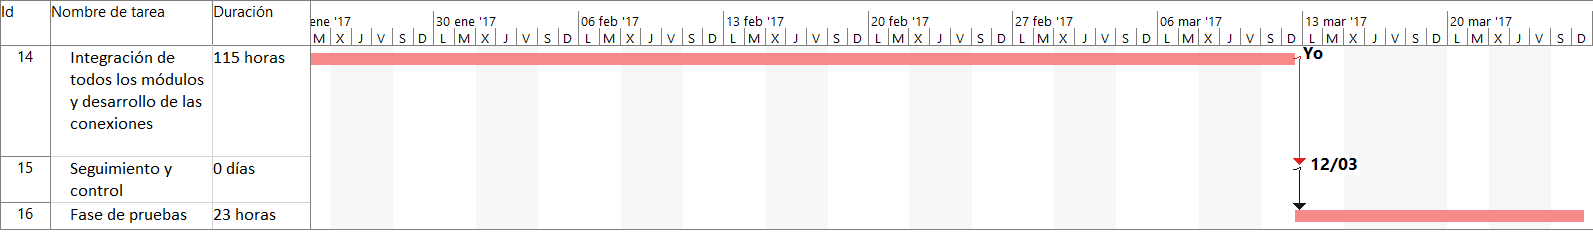
\includegraphics[angle=270,width=0.25\textwidth]{img/ganttFinal3}
	\caption{Diagrama de Gantt Final 3}
	\label{fig:ganttFinal3}
\end{figure}

\begin{figure}[H]
	\centering
	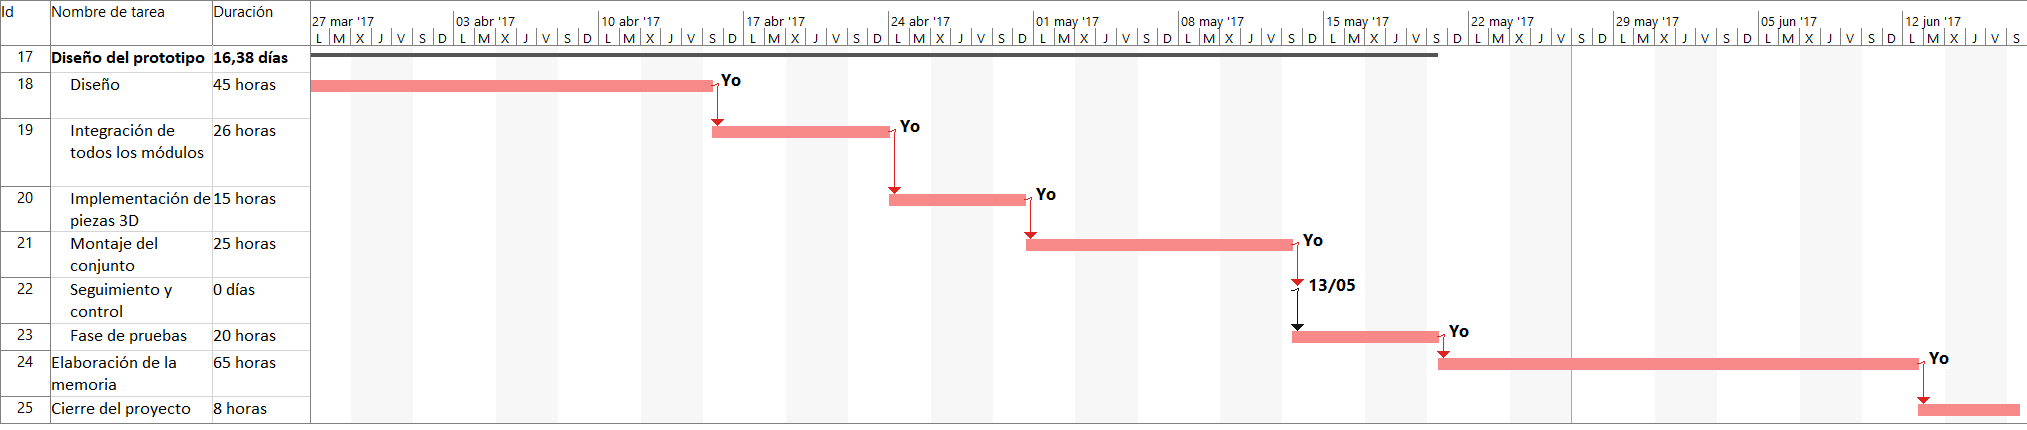
\includegraphics[angle=270,width=0.35\textwidth]{img/ganttFinal4}
	\caption{Diagrama de Gantt Final 4}
	\label{fig:ganttFinal4}
\end{figure}

\begin{figure}[H]
	\centering
	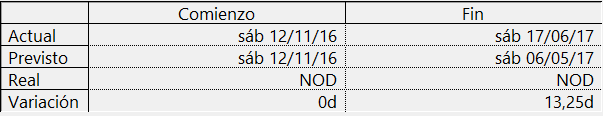
\includegraphics[width=0.7\textwidth]{img/variacionFechas}
	\caption{Esquema de variación de fechas}
	\label{fig:variacionFechas}
\end{figure}

\begin{figure}[H]
	\centering
	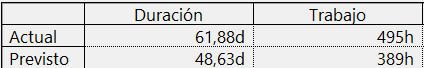
\includegraphics[width=0.7\textwidth]{img/variacionDuracion}
	\caption{Esquema de variación de la duración del proyecto}
	\label{fig:variacionDuracion}
\end{figure}

\begin{figure}[H]
	\centering
	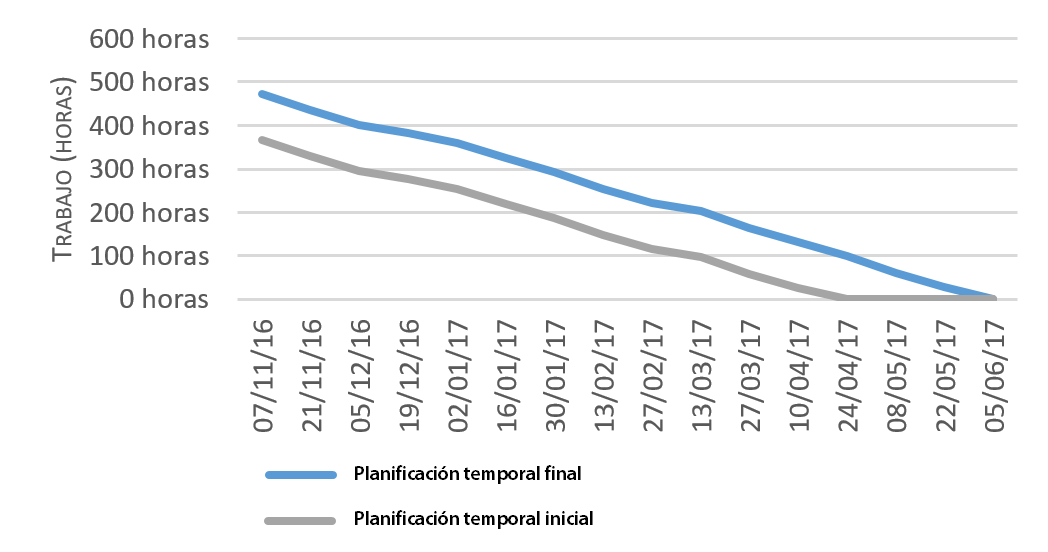
\includegraphics[width=0.7\textwidth]{img/graficaComparativaTiempo}
	\caption{Gráfica comparativa del trabajo previsto y real}
	\label{fig:graficaComparativa}
\end{figure}

\section{Planificación financiera final} 

A continuación detallaremos una planificación financiera a posteriori:
\begin{itemize}
	\item Modelo a escala de un buggy: 43,85 \euro
	\item Raspberry Pi 3 modelo B: 38,70 \euro
	\item Webcam: 15 \euro
	\item Variador (control motor): 9,66 \euro
	\item Arduino Nano: 4,40 \euro
	\item Servo: 2,60 \euro
	\item Placa para integrado: 0,37 \euro
	\item Macho-hembra integrado: 0,50 \euro
	\item Macho-macho integrado: 0,50 \euro
	\item Cables integrado: 1,00 \euro
	\item Clavijas conexión motor: 0,35 \euro
	\item Clavija conexión bateria: 1,20 \euro
	\item Cables interconexión: 2 \euro
	\item Placa impresa 3D: 13 \euro
	\item LEDS: 2,40 \euro
	\item Resistencias: 0,30 \euro
	\item Horas de trabajo: 495 h * 8 \euro/h = 3960 \euro

\fbox{Presupuesto total: 4095,83 \euro}
\end{itemize}

\section{Estudio de mercado}
\subsection{Clientes potenciales}

	En nuestro proyecto podemos barajar varios clientes potenciales.
	
	\begin{itemize}
		\item Para clientes amantes del modelismo.
		
			Como producto de modelismo podría tener una buena salida ya que es una nueva forma de entender el modelismo. Además suelen ser personas amantes de los nuevos productos, y podría llegar a convertirse en una nueva categoría de este.
			
			
		\item Para clientes a los que les gusta la programación y geeks.
			
			Suponemos que las personas que aquí contemplamos están en los grupos de ``Ciencias, matemáticas e informática'' e ``Ingeniería, industria y construcciones'' ya que son los más propensos a pertenecer a este tipo de clientes. Con ello, según el INE, en el año 2011 estos grupos eran el 8,7 \% y el 16,2 \% de la población respectivamente. Con ello nos da un 24,9 \% de la población que tienen la posibilidad de ser clientes potenciales. \cite{censoINE}
		
		\item Para automatización de coches.
		
			Tomando el censo de conductores de 2015 el número de conductores con el permiso de conducir de tipo B entre una edad de 18 y 40 años es de 7591503. La población en el año 2015 era aproximadamente de 46,62 Millones de personas. Con lo cual supuestamente tendríamos un 16,28 \% de la población que podrían ser clientes potenciales. \cite{censoDGT}
			
		
		\item Para automatización de vehículos extraterrestres.
		
			Alguna de las agencias espaciales podría necesitar este producto al ser un producto de bajo coste y fácilmente escalable y replicable. Podría utilizarse como ``cerebro'' para controlar vehículos que pudiesen ser enviados fuera de la tierra.
			
		
	\end{itemize}

\subsection{Plan de comercialización}

	En nuestro caso vamos a estudiar dos posibles maneras de comercializar el producto.

	\begin{itemize}
		\item Pack automatización
		
			En este caso se vendería las Raspberry, el Arduino, la placa que diseñamos y la cámara, además del software que esto incluye. En este caso el coste de las piezas por unidad suman 78,17 \euro a lo que deberíamos sumar las horas de trabajo para montar el hardware y el software en cada pieza que se estima en unas 40 horas de trabajo, con lo que suman 320 \euro. Al sumar nos sale un coste por unidad de 398,17 \euro a priori. 
			
			 Suponiendo que obtenemos un descuento de un 20 \% de descuento en el hardware por numero de unidades, nos queda un precio de materiales de 62,54 \euro más el coste del trabajo 320 \euro suman 382,64 \euro. A esto sumamos un 25 \% de beneficio y resulta 478,17 \euro. El coste final para el producto más IVA es de 578,59 \euro.
			 
			 En este caso, como podríamos estar hablando de automatización de coches, podemos suponer que un 5 \% de los clientes potenciales nos compran el Pack, con lo que venderíamos unas 380000 unidades aproximadamente. Con ello estaríamos hablando de 95,53 \euro/ud * 380000 ud = 36301400 \euro  de beneficio. Si a esto restamos el coste real de producción del primer prototipo quedaría 36301400 \euro  -  4095,83 \euro = 36297304,17 \euro  de beneficio.
			
		\item Coche hobby
		
			Por contra, aquí comercializaríamos el prototipo al completo. Entonces el coste material suman 135,83 \euro. A esto le sumamos el trabajo por montar un prototipo estimado en unas 75 h, lo que resulta 600 \euro. Con lo cual, a priori el coste por unidad es de 735,83 \euro.
			
			Suponiendo un descuento por unidades de un 20 \% en el hardware, nos resulta un costo en materiales de 108,67 \euro/ud. A esto le sumamos el costo de trabajo estimado en 600 \euro/ud. Con lo cual tenemos un coste de 708,67 \euro/ud. Además teniendo en cuenta un 25 \% de beneficio nos arroja 885,84 \euro/ud. Por tanto el coste total con IVA incluido es de 1071,84 \euro.
			
			Luego suponiendo unas ventas de 100000 ud, el beneficio asciende a 177,17 \euro/ud, con lo cual, un beneficio bruto total 100000 ud * 177,17 \euro/ud = 17717000 \euro. Si le restamos el coste del prototipo inicial 17717000 \euro - 4095,83 \euro = 17712904,17 \euro de beneficio.
		
	\end{itemize}
 
\cdpchapter{Conclusiones}

	Debido a la falta de tiempo como ya hemos comentado antes, no se han cumplido al 100 \% los objetivos. El primer objetivo ``Construir un coche radiocontrol controlado por una RaspberryPi'' se ha cumplido completamente y a la perfección.
	
	En cuanto al objetivo de automatización es donde más nos hemos alejado de la idea inicial. Lo que pensábamos hacer era que el coche mediante la cámara siguiera un circuito e incluso evitara obstáculos. Pero debido a la falta de tiempo sólo se pudo llegar a implementar la detección de personas, combinada con el control del coche.
	
	En conclusión, no solo ya conforme a la cobertura de los objetivos iniciales, que dentro de lo que cabo nos sentimos satisfechos del trabajo realizado, si no los conocimientos adquiridos sobre el manejo de las placas, el protocolo de comunicación serie, el protocolo de comunicación en red, etc. 


\cdpchapter{Trabajo futuro}

	En el futuro podría mejorarse como no lo que el tiempo no nos ha dejado terminar, la autonomía del coche, que el coche vaya solo con la cámara sin intervención de nadie. 
	
	También surgen líneas como la seguridad, la red WiFi que ahora mismo emite nuestra Raspberry es una red abierta, sin clave, con lo que cualquiera podría conectarse y trastear la placa. 
	
	Además podría mejorarse el protocolo de comunicación entre la Raspberry y los clientes, que aunque esté implementada sobre TCP, debería de haber comunicación en ambos sentidos para confirmar la correcta recepción de las órdenes.
	
	Si el proyecto continuase, además habría que plantearse que Raspberry se pudiese integrar en un sistema con comunicación CAN-BUS como el que utilizan la mayoría de los coches modernos, con lo que ganaríamos luego en facilidad de instalación en cualquier modelo de coche ya comercializado.


\cdpchapter{Bibliografía}
	
	\bibliographystyle{apacite}
	\bibliography{bibliografia} 
	


\cdpchapter{Anexos}





\begin{enumerate}[a)]
	\item Alojamiento del proyecto
	
		El proyecto ha ido siendo alojado en un repositorio de github para el control de versiones y para tener un respaldo online. Enlace: \url{https://github.com/gorocca/autonomousbuggypi}
	
	\item Vídeos de prueba
		\begin{itemize}
			\item Primer vídeo de prueba con la aplicación
				\begin{figure}[H]
					\centering
					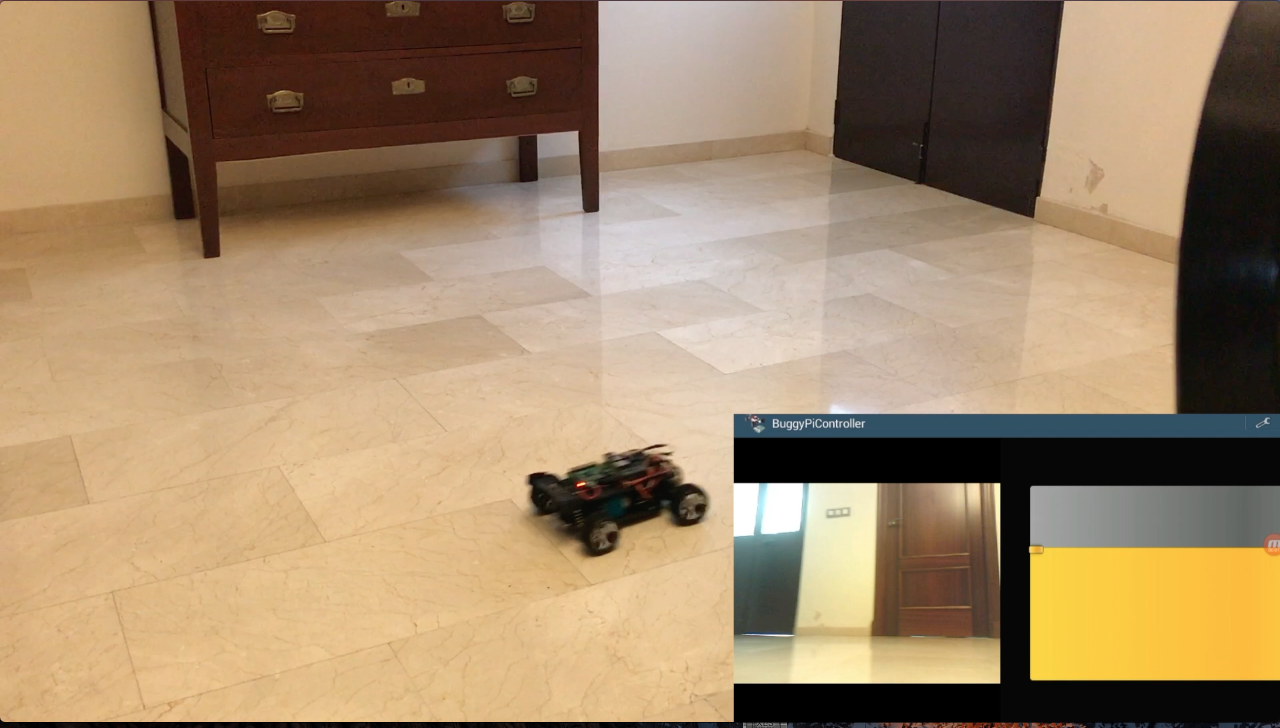
\includegraphics[width=0.7\textwidth]{img/capturaPrimerVideoApp}
					\caption{Captura del vídeo de prueba con la aplicación}
					\label{fig:capturaPrimerVideoApp}
				\end{figure}
		
				 Vídeo: \url{https://youtu.be/g_npEDxkSyo}
				
		\end{itemize}

\end{enumerate}



\end{document}

